% A Q&A chapter available in this template can help you when you want to change settings or need examples of how to get what you want.

\documentclass[	11pt,				% Font size
				twoside,			% Comment if you want to print on one side
				openright,
				headsepline,		% Adds a line under the page header
				headings=small,		% Defines sizing of the headers
				numbers=noenddot,	% No point at the right side of the section number
				%draft=false,
				BCOR=15mm,			% Absolute value of the binding correction.
				DIV=10, 			% larger value --> larger use of the page
				%captions=tableheading,
				paper=a4,			% only change if you want  another paper size
				abstracton,
				]{scrreprt}
				

%-----------------------------------------------------------------------------
% Document toggles for automatic adaptation of the document type
%-----------------------------------------------------------------------------
\usepackage{etoolbox}	% Makes it possible to really code in LaTeX
% Defining toggles
\newtoggle{dissertation}
\newtoggle{thesis}
\newtoggle{ingerman}
\newtoggle{inenglish}
\newtoggle{nobinding}
\newtoggle{boldcaptions}

%%%%%%%%%%%%%%%%%%%%%%%%%%%%%%%%%%%%%%%%%%%%%%%%%%%%%%%%%%%%%%%%%%%%%%%%%%%%%%%%%%%%%%%%%%%% 
%TODO Setting values for toggles - Change here to modify the document layout to your needs %
%%%%%%%%%%%%%%%%%%%%%%%%%%%%%%%%%%%%%%%%%%%%%%%%%%%%%%%%%%%%%%%%%%%%%%%%%%%%%%%%%%%%%%%%%%%%

%%% Main properties %%%
\togglefalse{dissertation}		%if true (\toggletrue{dissertation}): no cover page
\toggletrue{thesis}				%if true (\toggletrue{thesis}): master or bachelor thesis (set false if \toggletrue{dissertation})
\togglefalse{ingerman}			%if \toggletrue{ingerman}: german if \togglefalse{ingerman}: english

%%% Secondary properties %%% 
\togglefalse{nobinding}		%if true: page layout is centered	
\toggletrue{boldcaptions}  	%if true: Fig. and Tab. are bold

%For oneside print: comment twoside in documentclass (line 4)






%%%%%%%%%%%%%%%%%%%%%%%%%%%%%%%%%%%%%%%%%
%%%% Settings - depending on toggles %%%%

%-----------------------------------------------------------------------------
% Language selection and translation definitions
%-----------------------------------------------------------------------------
% Depending on if german is selected as the main language, this part defines the main and secondary languages in the document and defines correct titles accordingly.
\iftoggle{ingerman}{%
	\newcommand{\mainLanguage}{ngerman}
	\newcommand{\secondLanguage}{english}
	\newcommand{\abstractMain}{Kurzfassung}
	\newcommand{\abstractSecond}{Abstract}
	\newcommand{\listOfFigures}{Abbildungsverzeichnis}
	\newcommand{\listOfTables}{Tabellenverzeichnis}
	\newcommand{\nomenclatureName}{Nomenklatur}
	\newcommand{\appendixName}{Anhang}
	\newcommand{\GreekSymbols}{Griechische Formelzeichen}
	\newcommand{\RomanSymbols}{Formelzeichen und Einheiten}
	\newcommand{\abbreviations}{Abk\"urzungen}
	\newcommand{\subscripts}{Indizes}
	\newcommand{\Literaturename}{Literaturverzeichnis}
}{%
	\newcommand{\mainLanguage}{english}
	\newcommand{\secondLanguage}{ngerman}
	\newcommand{\abstractMain}{Abstract}
	\newcommand{\abstractSecond}{Kurzfassung}
	\newcommand{\listOfFigures}{List of Figures}
	\newcommand{\listOfTables}{List of Tables}
	\newcommand{\nomenclatureName}{Nomenclature}
	\newcommand{\appendixName}{Appendix}
	\newcommand{\GreekSymbols}{Greek Symbols}
	\newcommand{\RomanSymbols}{Roman Symbols}
	\newcommand{\abbreviations}{Abbreviations}
	\newcommand{\subscripts}{Subscripts}
	\newcommand{\Literaturename}{Literature}
}


%-----------------------------------------------------------------------------
% Page layout (margins, headers and footers)
%-----------------------------------------------------------------------------
\usepackage{geometry}
%\usepackage{scrlayer-scrpage} % Package to control headers and footers more comprehensive
%\pagestyle{scrheadings} % To automatically format headers and footers well when having two page print and different left and right margins

\newtoggle{onesideprint}
\makeatletter
	\if@twoside
		\togglefalse{onesideprint}
	\else
		\toggletrue{onesideprint}
	\fi
\makeatother

\interfootnotelinepenalty=10000 % Prevents the footnotes to split in two pages

\newlength{\lmargin}
\newlength{\rmargin}
\newlength{\tmargin}
\newlength{\bmargin}

% Defining page margins for different document types
	%page width
\iftoggle{nobinding}{
	\iftoggle{dissertation}{
		\setlength{\lmargin}{27mm}
		\setlength{\rmargin}{27mm}
	}{}
	\iftoggle{thesis}{
		\setlength{\lmargin}{27.5mm}
		\setlength{\rmargin}{27.5mm}
	}{}
}{	\iftoggle{onesideprint}{                % If with binding and one page print
		\iftoggle{dissertation}{
			\setlength{\lmargin}{30mm}
			\setlength{\rmargin}{24mm}
		}{}
		\iftoggle{thesis}{
			\setlength{\lmargin}{30mm}
			\setlength{\rmargin}{25mm}
		}{}
		}{                                  % If with binding and two page print
		\iftoggle{dissertation}{
			\setlength{\lmargin}{24mm}
			\setlength{\rmargin}{30mm}
		}{}
		\iftoggle{thesis}{
			\setlength{\lmargin}{30mm}
			\setlength{\rmargin}{25mm}
	}{}}
}
	%page height
\iftoggle{dissertation}{
	\setlength{\tmargin}{35mm}
	\setlength{\bmargin}{35mm}
}{}
\iftoggle{thesis}{
	\setlength{\tmargin}{37mm}
	\setlength{\bmargin}{38mm}
}{}

% Setting the page margins
\geometry{a4paper, left=\lmargin, right=\rmargin, top=\tmargin, bottom=\bmargin}

\newlength{\offsetCoverPage}
\newlength{\marginCoverPage}
\iftoggle{onesideprint}{%
	\setlength{\offsetCoverPage}{-1mm}
	\setlength{\marginCoverPage}{0mm}

}{%
	\setlength{\offsetCoverPage}{0mm}
	\setlength{\marginCoverPage}{0.25mm}
}

%% Setting header and footers
\usepackage{fancyhdr}	% This package is easier to control than the already implemented header and footer controls in the Koma-Script class
\pagestyle{fancy}

\renewcommand{\sectionmark}[1]{\normalsize\markright{\thesection\ #1}{}}
\renewcommand{\chaptermark}[1]{\normalsize\markboth{\thechapter\ #1}{}}
\lhead{\leftmark}
\chead{}
\rhead{\rightmark}

%-----------------------------------------------------------------------------
% Base packages
%-----------------------------------------------------------------------------
\usepackage[T1]{fontenc}	 % Enables font encoding for accented characters
\usepackage[utf8]{inputenc}  % Enables input of accented characters
\usepackage[english,ngerman]{babel}	% Defines the document language
\usepackage{ifpdf} 		
% This creates a true boolean if you are executing your code using PDFLatex or LuaLaTex, otherwise it is false. It helps later on to define correct package options for different compiling methods. (See PDF-Setup)

\usepackage{blindtext} % Just to create lorem ipsum text in this template
\usepackage{datetime}
\newdateformat{monthyeardate}{%
  \monthname[\THEMONTH] \THEYEAR}

% There exist several todo packages like todonotes, todo, or easy-todo.
% Choose one todo package and import it via the \usepackage{} command.

%-----------------------------------------------------------------------------
% Font properties
%-----------------------------------------------------------------------------
%\usepackage{fourier} %PDF-compatible font "Utopia". There exists a free look-alike: Heuristica
\usepackage{lmodern} % So that headings don't pixelate (bitmap font to vector font); Don't use it simultaneously with fourier (previous font, see more at issues 16 and 20)
\makeatletter % No warnings because of a replaced font
  \let\@font@info\@gobble
  \let\@font@warning\@gobble
\makeatother

\iftoggle{boldcaptions}{
	\renewcommand{\caplabelfont}{\bfseries} % Fig. and Tab. are bold
}{}


%-----------------------------------------------------------------------------
% Redefining bullet points
%-----------------------------------------------------------------------------
\AtBeginDocument{
  \renewcommand{\labelitemi}{\(\bullet\)}
  \renewcommand{\labelitemii}{\(\circ\)}
}


%-----------------------------------------------------------------------------
% Line and paragraph spacing
%-----------------------------------------------------------------------------
\usepackage{setspace} % Change Linespread
\onehalfspacing % Linespread 1.5
\setlength\parskip{\medskipamount} % Small linespread between two paragraphs
\setlength\parindent{0pt} % No indentation in the first line of a new paragraph


%-----------------------------------------------------------------------------
% Color definitions
%-----------------------------------------------------------------------------
\usepackage{xcolor}
% The standart ERC colors (dark variant)
% Check sharepoint for lighter variants if needed
\definecolor{ercred}{RGB}{229,48,39}	% Color of the ERC logo
\definecolor{ercblue}{RGB}{16, 88, 176}
\definecolor{ercorange}{RGB}{244, 115, 40}
\definecolor{ercviolett}{RGB}{95, 55, 155}
\definecolor{ercdarkred}{RGB}{155, 35, 30}
\definecolor{ercpink}{RGB}{190, 65, 152}
\definecolor{ercdarkgreen}{RGB}{0, 135, 70}
\definecolor{ercgray}{RGB}{120, 120, 120}
\definecolor{ercredPics}{RGB}{221,64,45}

% The official RWTH colors
% Check official document for lighter colors if needed
\definecolor{rwthblue}{RGB}{0,84,159}
\definecolor{rwthblack}{RGB}{0,0,0}
\definecolor{rwthmagenta}{RGB}{227,0,102}
\definecolor{rwthyellow}{RGB}{255,237,0}
\definecolor{rwthpetrol}{RGB}{0,97,101}
\definecolor{rwthturquoise}{RGB}{0,152,161}
\definecolor{rwthgreen}{RGB}{87,171,39}
\definecolor{rwthmaygreen}{RGB}{189,205,0}
\definecolor{rwthorange}{RGB}{246,168,0}
\definecolor{rwthred}{RGB}{204,7,30}
\definecolor{rwthbordeaux}{RGB}{161,16,53}
\definecolor{rwthviolett}{RGB}{97,33,88}
\definecolor{rwthlila}{RGB}{122,11,172}

% Color aliases
% Use these in the document to be able to switch easily
\colorlet{color0}{ercred}
\colorlet{color1}{ercblue}
\colorlet{color2}{ercorange}
\colorlet{color3}{ercviolett}
\colorlet{color4}{ercdarkred}
\colorlet{color5}{ercpink}
\colorlet{color6}{ercdarkgreen}

%-----------------------------------------------------------------------------
% List environments
%-----------------------------------------------------------------------------
\usepackage{enumitem}
% This provides more user control over the list environments. Here you can create your own enumeration format, etc. (See Q&A Environment Setup as an example)


%-----------------------------------------------------------------------------
% Style formats 
%-----------------------------------------------------------------------------
\usepackage{listings}
% This enables writing programming code as written in a programming environment in LaTeX.

\lstset{literate=%
    {ä}{{\"a}}1
    {Ä}{{\"A}}1
    {ö}{{\"o}}1
    {Ö}{{\"O}}1
    {ü}{{\"u}}1
    {Ü}{{\"Ü}}1
    {ß}{{\ss}}1
}
% Adds the possibility to include german special charachters in the lstlisting.

\usepackage{textcomp} % Is needed, if "\usepackage{lmodern}" is used (Line 195)
\usepackage{Resources/ModelicaStyle}	% Modelica style file

%-----------------------------------------------------------------------------
% Nomenclature
%-----------------------------------------------------------------------------
\usepackage[intoc]{nomencl}		% Used for automatic generation of nomenclature
\RequirePackage{ifthen}			% Checks if ifthen functions
% Defines the nomenclature sections
\renewcommand{\nomgroup}[1]{%
	\ifthenelse{\equal{#1}{G}}{\item[\newline\textbf{\GreekSymbols}]}{
	\ifthenelse{\equal{#1}{U}}{\item[\newline\textbf{\subscripts}]}{
	\ifthenelse{\equal{#1}{A}}{\item[\newline\textbf{\abbreviations}]}{
	\ifthenelse{\equal{#1}{S}}{\item[\newline\textbf{\RomanSymbols}]}{
	\ifthenelse{\equal{#1}{Y}}{\item[\newline\textbf{Codes used for configurations of simulation}]}{
}}}}}
}
% Changing some of the spacings
\newcommand{\nomunit}[1]{%
\renewcommand{\nomentryend}{\hspace*{\fill}#1}%
}
\renewcommand{\nomlabel}[1]{\hspace{2.5em}#1}
\makenomenclature
\setlength\nomlabelwidth{2.5cm}


%-----------------------------------------------------------------------------
% Mathematic
%-----------------------------------------------------------------------------
\usepackage{amsmath}
\usepackage{amssymb}
\usepackage{array}
\DeclareMathAlphabet\mathbfcal{OMS}{cmsy}{b}{n}
%-----------------------------------------------------------------------------
% Q&A environment setup
%-----------------------------------------------------------------------------
% The following commands are only used for the Q&A format in the examples of the template. You can remove this in your main document. Note that this is also useful for cerating exam formats, etc.
%\newenvironment{QandA}{\begin{enumerate}[label=\bfseries\arabic*.]\bfseries}
%                      {\end{enumerate}}
%\newenvironment{answered}{\par\normalfont}{}


%-----------------------------------------------------------------------------
% PDF-Setup
%-----------------------------------------------------------------------------
\ifpdf
	%We use PDFLaTeX
	\usepackage[pdftex]{graphicx} 
	\pdfimageresolution=100
	\pdfminorversion=7
	\pdfcompresslevel=9
	\usepackage[pdftex,
		urlcolor=blue,
		linktoc=all,
		colorlinks=true,
		linkcolor=black,
		citecolor=black,
		pdfview=FitH,
		pdfstartview=FitH,
		plainpages=false]{hyperref}	% Allows cross references and hyperlinks
	\hypersetup{
		pdfauthor={Your Name here},
        pdftitle={Name of your thesis},
        pdfsubject={},
        pdfkeywords={several helpful keywords},
        pdfproducer={LaTeX with hyperref},
        pdfcreator={pdflatex}}
    \usepackage[figure,figure*]{hypcap}
\else
	%DVI oder PS Ausgabe
	\usepackage{graphicx} 
\fi
\usepackage{pdfpages}	
% Simplifies the inclusion of whole PDF-Pages, e.g. cover page. Should be placed after "graphicx" package


%-----------------------------------------------------------------------------
% Units and symboles
%-----------------------------------------------------------------------------
\usepackage{siunitx}	
% Prefered to package "siunits". Should be placed after "graphicx" package

\usepackage[official]{eurosym}
\DeclareUnicodeCharacter{20AC}{\euro} 
% The normale euro symbol via [Alt Gr][€] is replaced by a high quality one

%-----------------------------------------------------------------------------
% General floats
%-----------------------------------------------------------------------------
\usepackage{float}
\usepackage{placeins}	% Allows more control of the floats, e.g. \FloatBarrier
\usepackage{caption}	
\usepackage{subcaption}	% Allows manipulation of caption entries in lists

%-----------------------------------------------------------------------------
% Figures
%-----------------------------------------------------------------------------
\graphicspath{{Figures/}}	% Defining where the figure are located (for pdf_tex).

\usepackage{tikz,pgfplots} \pgfplotsset{compat=newest}
% Allows using TikZ plots with the newest package available
\usetikzlibrary{plotmarks, shapes, arrows, positioning, shadows, trees}
% plotmarks is used in the diagrams, other values are for flow charts, etc.

%\usetikzlibrary{external}	% Uncomment to activate external TikZ compliation
%\tikzexternalize[prefix=Figures/TikZ]	% Uncomment to place external tikZ files in a separate folder.

\newlength\figureheight 
\newlength\figurewidth 
% Defining the length and height variables of the TikZ plots


%-----------------------------------------------------------------------------
% Tables
%-----------------------------------------------------------------------------
\usepackage{longtable}	% For tables longer than a page
\usepackage{multirow}	% Allows multirow in tables
\usepackage{multicol}	% Allows multicolumn in tables
\usepackage{booktabs}	% Better horizontal lines in tables \toprule \midrule ...

\usepackage{dcolumn} 	% Allows allignment by decimal point
  \newcolumntype{d}[1]{D{.}{.}{#1}}	% Defining some new formats
  \newcolumntype{C}[1]{>{\centering\let\newline\\\arraybackslash\hspace{0pt}}m{#1}}



%-----------------------------------------------------------------------------
% References and Citations
%-----------------------------------------------------------------------------
%\usepackage{varioref}
\usepackage[square,numbers]{natbib}
%\usepackage{bibunits}


%-----------------------------------------------------------------------------
% Manually added packages
%-----------------------------------------------------------------------------
\usepackage{ziffer}


%%%%%%%%%%%%%%%%%%%%%%%%%%%%%%%%%%%%%%%%%%%%%%%%%%%%%%%%%%%%%%%%%%%%%%%%%%%%%%
%-----------------------------------------------------------------------------
% DOCUMENT BEGINS HERE!
%-----------------------------------------------------------------------------
%%%%%%%%%%%%%%%%%%%%%%%%%%%%%%%%%%%%%%%%%%%%%%%%%%%%%%%%%%%%%%%%%%%%%%%%%%%%%%

\begin{document}


\pagestyle{empty}
\newcounter{Hilfszaehler}

\expandafter\selectlanguage\expandafter{\mainLanguage}

\cleardoublepage
\pagenumbering{Roman} % roman page numbers


%-----------------------------------------------------------------------------
% Cover page
%-----------------------------------------------------------------------------
% Based on the document type and language, the template decides if and which cover page should be used and includes it in the final document.

\includepdf{Chapters/Deckblatt_MA.pdf}
\iftoggle{thesis}{%
	\iftoggle{ingerman}{%
		\begin{titlepage}
	\begin{addmargin}{\offsetCoverPage} 
		%TODO Um das RWTH-Logo zu benutzen, musst du das Formblatt RWTH-Logo Deutsch aus der Datei Formulare.txt
		%TODO ausfüllen und es dem ZPA schicken!
		
		%-----------------------------------------------------------------------------
		% Platzierung der Kopfzeile(Nummer und Logo)
		%-----------------------------------------------------------------------------
		\setlength{\unitlength}{1cm}
		\begin{picture}(0,0)
			%\put(7.977,0){
\includegraphics[width = 0.5\textwidth]{Resources/HMTM-Logo-2010}}
			%TODO Ändere die Nummer deiner Arbeit, und wenn noetig die Bezeichnung(BA, MA, PA)
			%TODO Die Abkürzungen sind Deutsch, auch wenn die Arbeit in Englisch verfasst wird
			%\put(0,1.32){\fontfamily{phv}\selectfont\huge{MA 508}}
		\end{picture}
		\begin{center}
			{\scshape\LARGE Hochschule für Musik und Tanz Köln\par}
		\end{center}\centering
	
	\end{addmargin}
%-----------------------------------------------------------------------------
% Titel deiner Arbeit
%-----------------------------------------------------------------------------
		\addvspace{2.6cm}
		%TODO Formaenderung des Titels
		\begin{addmargin}[\marginCoverPage]{0cm}
			\begin{center}
				{\scshape\Large Masterarbeit\par}
			\end{center}
			
	\vspace{1.5cm}
	{\huge\bfseries Entwicklung musikalischer Fähigkeiten von Senior*innen\par}



%-----------------------------------------------------------------------------
% Namen, Daten
%-----------------------------------------------------------------------------
\vfill
\begin{center}
\begingroup
\fontfamily{phv}\selectfont
%TODO Bitte aendere das Datum deiner Abgabe
Köln, \monthyeardate\today \\
\addvspace{0.5cm}
%TODO Bitte aendere deinen Namen und Matrikelnummer in den naechsten beiden Zeilen
\textbf{Hannah Marie Losch} \\
Matrikelnummer: 108588 \\
\addvspace{0.5cm}
%TODO Deine Betreuer. Achte auf die richtige Schreibweise des Titels.
Betreuer:\\
Dr. Florian Worschech \\
Prof. Dr. Hans Neuhoff\\
\addvspace{0.5cm}
%TODO  Eingabe der richtigen Anschrift des Instituts.
Diese Arbeit wurde vorgelegt am:\\
HMTM Hannover \\
Institut für Musikermedizin und Musikphysiologie\\
Neues Haus 1, 30175 Hannover\\
\endgroup
\end{center}
\end{addmargin}
\end{titlepage}


	}%{%
		\begin{titlepage}
	\begin{addmargin}{\offsetCoverPage} 
		%TODO Um das RWTH-Logo zu benutzen, musst du das Formblatt RWTH-Logo Deutsch aus der Datei Formulare.txt
		%TODO ausfüllen und es dem ZPA schicken!
		
		%-----------------------------------------------------------------------------
		% Platzierung der Kopfzeile(Nummer und Logo)
		%-----------------------------------------------------------------------------
		\setlength{\unitlength}{1cm}
		\begin{picture}(0,0)
			%\put(7.977,0){
\includegraphics[width = 0.5\textwidth]{Resources/HMTM-Logo-2010}}
			%TODO Ändere die Nummer deiner Arbeit, und wenn noetig die Bezeichnung(BA, MA, PA)
			%TODO Die Abkürzungen sind Deutsch, auch wenn die Arbeit in Englisch verfasst wird
			%\put(0,1.32){\fontfamily{phv}\selectfont\huge{MA 508}}
		\end{picture}
		\begin{center}
			{\scshape\LARGE Hochschule für Musik und Tanz Köln\par}
		\end{center}\centering
	
	\end{addmargin}
%-----------------------------------------------------------------------------
% Titel deiner Arbeit
%-----------------------------------------------------------------------------
		\addvspace{2.6cm}
		%TODO Formaenderung des Titels
		\begin{addmargin}[\marginCoverPage]{0cm}
			\begin{center}
				{\scshape\Large master thesis\par}
			\end{center}
			
	\vspace{1.5cm}
	{\huge\bfseries Musical Development of Healthy Older Adults \par}

\addvspace{1cm}
\begin{center}
	%TODO Falls der deutsche Name noch noetig ist, kommt er in die naechste Zeile
	{\Large A Randomized Controlled Trial Assessing Piano Progress over 12 Months of Instruction}
\end{center}


%-----------------------------------------------------------------------------
% Namen, Daten
%-----------------------------------------------------------------------------
\vfill
\begin{center}
\begingroup
%\fontfamily{phv}\selectfont
%TODO Bitte aendere das Datum deiner Abgabe
Köln, \monthyeardate\today \\
\addvspace{0.5cm}
%TODO Bitte aendere deinen Namen und Matrikelnummer in den naechsten beiden Zeilen
\textbf{Hannah Marie Losch} \\
108588 \\
\addvspace{0.5cm}
%TODO Deine Betreuer. Achte auf die richtige Schreibweise des Titels.
Supervisor:\\
Dr. Florian Worschech \\
Prof. Dr. Hans Neuhoff\\
\addvspace{0.5cm}
%TODO  Eingabe der richtigen Anschrift des Instituts.
HMTM Hannover \\
Institut für Musikermedizin und Musikphysiologie\\
Neues Haus 1, 30175 Hannover\\
\endgroup
\end{center}
\end{addmargin}
\end{titlepage}


	%}
}{}
%\iftoggle{dissertation}{%
%	\input{Chapters/Promotion_cover_page_promotionsgesuch.tex}
%	\input{Chapters/Promotion_cover_page_publication.tex}
%}
\newpage 
\thispagestyle{empty}
\quad 
\newpage

%-----------------------------------------------------------------------------
% Page numbers
%-----------------------------------------------------------------------------
\pagenumbering{Roman} % roman page numbers

\iftoggle{onesideprint}{
	\fancyfoot[C]{\thepage}
	\fancyfoot[LE,RO]{}}
	{
	\fancyfoot[LE,RO]{\thepage}
	\fancyfoot[C]{}
	}

%-----------------------------------------------------------------------------
% Abstract in English and German (Both are required)
%-----------------------------------------------------------------------------
% Different documents have different types of showing the title of the abstract, This part assigns the correct formmat to your document considering the main and secondary language.
\refstepcounter{Hilfszaehler}
\iftoggle{thesis}{%
	\begin{abstract}
		Background: Although the literature has demonstrated that older people are generally still capable of learning new motor skills \cite{Boyke2008, Anguera2013, Altenmuller2020}, the development of musical skills in older people is poorly studied. The present experiment aimed to examine the development of musical abilities in the aging population and to identify factors that contribute to the development of these skills.

Methods: A cohort of 72 elderly participants (age = 69.5 years ± 3.14) from Hannover and Geneva without prior musical practice participated in a 12-month piano training program with weekly lessons. Participants’ piano performance was audibly assessed at 3 and 12 months of intervention and subsequently rated by unrelated piano students (holding at least a bachelor’s degree) with teaching experience. Each rater evaluated the piano performance of each participant blindly and in randomized order, considering articulation, dynamics, rhythm, pitch, fluency and expressivity on a scale from 1 to 7. Various predictors such as age, gender, education, and musical sophistication were considered as potential predictors of individual progress.

Results: Bayesian statistical analysis of the data show that after three months of practice, younger participants with higher CogTel scores and more cognitive reserve achieve higher results in rhythm, fluency and pitch. In articulation (0.29, CI 95\%: [0.08, 0.51]) and dynamics (0.12, CI 95\%: [-0.01, 0.42]) a clear time effect over the course of the intervention can be observed. Especially younger participants with less cognitive reserve and those who claim to have less musical sophistication (such as musical emotions, singing abilities and engagement in musical activities) show greater improvement in their skills over time, catching up to or even surpassing participants who initially performed better.

Discussion: The findings of this study have the potential to advance our understanding of the development of musical skills in elderly individuals and contribute to the development of tailored approaches to promote musical engagement in this population. By identifying the factors that contribute to improved musical training outcomes, targeted interventions can be designed to optimize musical training strategies for older adults.
	\end{abstract}
	%\expandafter\selectlanguage\expandafter{\secondLanguage}
	%\begin{abstract}
		%The federal government's targets state that Germany should become greenhouse gas neutral by 2045. In 2021, 15\,\% of greenhouse gas emissions in Germany were attributable to the building sector. Innovations in the Building Energy Act and the federal government's requirement to install $500.000$ of new heat pumps every year from 2024 increase the demand for heat pumps.

In 2022, $86,9\,\%$ of the $236.000$ installed heat pumps in Germany were air-water heat pumps, as the investment costs are low compared to heat pumps with other energy sources. Air-to-water heat pumps may experience frosting on the heat exchanger in certain weather conditions, which reduces the Coefficient of Performance of the heat pump. To restore the efficiency of the heat pump, an energy-intensive defrosting process is necessary. The average Coefficient of Performance of the heat pump depends on the defrosting time. By determining optimal defrosting times, the efficiency of the heat pump can be increased. In most commercial heat pumps, the defrosting process is initiated in a time-controlled manner. Demand-based defrost controls are proposed in the literature, which often require additional sensor technology. One example is a control that measures the pressure loss of the air flow at the evaporator and initiates the defrosting process when a threshold value is exceeded.

In this work, a Reinforcement Learning agent for determining optimal defrosting times is developed and tested on an air-to-water heat pump. Since large amounts of data are necessary for the training, training data are generated in a heuristic simulation. An RL agent is developed that is able to abstract the optimisation problem from the simulation and project it onto real test bench data. This is followed by an experimental validation on a Hardware-in-the-Loop test bench at the E.ON Energy Research Center at RWTH Aachen University. Three dynamic 24-h tests with different frost growth rates are carried out. The validation is carried out by comparing a time-based controller (R1), a pressure difference-based controller (R2) designed according to literature recommendations and an optimised pressure difference-based controller (R3). Compared to R1, the average Coefficient of Performance of the RL controller is $7,1\,\%$ higher for fast frost growth, but $0,7\,\%$ lower for slow frost growth. Compared to R2, the average Coefficient of Performance of the RL controller is better between $3,3\,\%$ and $9,1\,\%$. Only R3 is more efficient than the RL control at slow frost growth up to~$2\,\%$.
 
	%\end{abstract}
	%\expandafter\selectlanguage\expandafter{\mainLanguage}
}{}
\iftoggle{dissertation}{%	
	\chapter*{\abstractMain}	
	Background: Although the literature has demonstrated that older people are generally still capable of learning new motor skills \cite{Boyke2008, Anguera2013, Altenmuller2020}, the development of musical skills in older people is poorly studied. The present experiment aimed to examine the development of musical abilities in the aging population and to identify factors that contribute to the development of these skills.

Methods: A cohort of 72 elderly participants (age = 69.5 years ± 3.14) from Hannover and Geneva without prior musical practice participated in a 12-month piano training program with weekly lessons. Participants’ piano performance was audibly assessed at 3 and 12 months of intervention and subsequently rated by unrelated piano students (holding at least a bachelor’s degree) with teaching experience. Each rater evaluated the piano performance of each participant blindly and in randomized order, considering articulation, dynamics, rhythm, pitch, fluency and expressivity on a scale from 1 to 7. Various predictors such as age, gender, education, and musical sophistication were considered as potential predictors of individual progress.

Results: Bayesian statistical analysis of the data show that after three months of practice, younger participants with higher CogTel scores and more cognitive reserve achieve higher results in rhythm, fluency and pitch. In articulation (0.29, CI 95\%: [0.08, 0.51]) and dynamics (0.12, CI 95\%: [-0.01, 0.42]) a clear time effect over the course of the intervention can be observed. Especially younger participants with less cognitive reserve and those who claim to have less musical sophistication (such as musical emotions, singing abilities and engagement in musical activities) show greater improvement in their skills over time, catching up to or even surpassing participants who initially performed better.

Discussion: The findings of this study have the potential to advance our understanding of the development of musical skills in elderly individuals and contribute to the development of tailored approaches to promote musical engagement in this population. By identifying the factors that contribute to improved musical training outcomes, targeted interventions can be designed to optimize musical training strategies for older adults.
	\expandafter\selectlanguage\expandafter{\secondLanguage}
	\chapter*{\abstractSecond}
	The federal government's targets state that Germany should become greenhouse gas neutral by 2045. In 2021, 15\,\% of greenhouse gas emissions in Germany were attributable to the building sector. Innovations in the Building Energy Act and the federal government's requirement to install $500.000$ of new heat pumps every year from 2024 increase the demand for heat pumps.

In 2022, $86,9\,\%$ of the $236.000$ installed heat pumps in Germany were air-water heat pumps, as the investment costs are low compared to heat pumps with other energy sources. Air-to-water heat pumps may experience frosting on the heat exchanger in certain weather conditions, which reduces the Coefficient of Performance of the heat pump. To restore the efficiency of the heat pump, an energy-intensive defrosting process is necessary. The average Coefficient of Performance of the heat pump depends on the defrosting time. By determining optimal defrosting times, the efficiency of the heat pump can be increased. In most commercial heat pumps, the defrosting process is initiated in a time-controlled manner. Demand-based defrost controls are proposed in the literature, which often require additional sensor technology. One example is a control that measures the pressure loss of the air flow at the evaporator and initiates the defrosting process when a threshold value is exceeded.

In this work, a Reinforcement Learning agent for determining optimal defrosting times is developed and tested on an air-to-water heat pump. Since large amounts of data are necessary for the training, training data are generated in a heuristic simulation. An RL agent is developed that is able to abstract the optimisation problem from the simulation and project it onto real test bench data. This is followed by an experimental validation on a Hardware-in-the-Loop test bench at the E.ON Energy Research Center at RWTH Aachen University. Three dynamic 24-h tests with different frost growth rates are carried out. The validation is carried out by comparing a time-based controller (R1), a pressure difference-based controller (R2) designed according to literature recommendations and an optimised pressure difference-based controller (R3). Compared to R1, the average Coefficient of Performance of the RL controller is $7,1\,\%$ higher for fast frost growth, but $0,7\,\%$ lower for slow frost growth. Compared to R2, the average Coefficient of Performance of the RL controller is better between $3,3\,\%$ and $9,1\,\%$. Only R3 is more efficient than the RL control at slow frost growth up to~$2\,\%$.
 
	\expandafter\selectlanguage\expandafter{\mainLanguage}
}{}

%-----------------------------------------------------------------------------
% Table of content
%-----------------------------------------------------------------------------
\cleardoublepage
\iftoggle{ingerman}{%
	\renewcommand{\contentsname}{Inhaltsverzeichnis}
}{%
	\renewcommand{\contentsname}{Table of Contents}
}

\pdfbookmark{\contentsname}{toc} % Link in PDF's bookmarks to TOC
%\setcounter{secnumdepth}{2}
\setcounter{tocdepth}{2}
\tableofcontents


%-----------------------------------------------------------------------------
% Nomenclature
%-----------------------------------------------------------------------------
% You can either add a long table as the nomenclature or use the "nomencl" package. The advantage of the long table is that you have more control on how it looks at the end while the disadvantages are that you have to sort everything manually and there is no possibility to add individual definitions in between the text. The "nomencl" package automatically creates the nomenclature based on definitions within the complete document. The disadvantage is you have to run <MakeIndex> during compilation. More info follows.
%\cleardoublepage
%\refstepcounter{Hilfszaehler}
%\addcontentsline{toc}{chapter}{\nomenclatureName}

%% The long table method ... (uncomment here and comment the next part)
%\pagestyle{plain}
%\chapter*{Nomenklatur}
\begin{onehalfspacing}
\begin{longtable}[h]{p{0.15\textwidth} p{0.55\textwidth} p{0.2\textwidth}}
		\caption*{\textbf{Formelzeichen und Einheiten}} \\
		\\
		\textbf{Symbol} & \textbf{Bedeutung} & \textbf{Einheit} \\ %\hline 
		\endhead
		\\
		\multicolumn{3}{c}{Fortsetzung auf der nächsten Seite} \\
		\endfoot
		\multicolumn{3}{c}{ } \\
		\endlastfoot
		$a$& Aktion&\\
		$A$& Fläche&$\mathrm{m}^2$\\
		$\vec a$&Aktivierung&\\
		$\mathcal{A}$&Aktionsraum&\\
		$b$&Bias&\\		
		$c_\mathrm{p}$ & isobare Wärmekapazität&J(kgK)$^{-1}$\\
		$c$& Konzentration&\si{\kilogram}\textsubscript{W}~ \si{\meter}$_\mathrm{L}^{-3}$\\
		$COP$ & Leistungszahl (engl.: \textit{Coefficient of Performance})& \\
		$d$& binärer Indikator (engl.: \textit{done})&\\
		$f$&Reifbildungsfaktor&\\
		$g$& Stoffübergangskoeffizient&kg m$^{-2}$\\
		$G$& Ertrag&\\
		$h$ & Enthalpie&\si{J}~\si{\kg}\textsuperscript{-1}\\
		$i$& Information&\\
		$j$& Parameter&\\
		$k$&Wärmeduchgangskoeffizient&m$^2$K W$^{-1}$\\
		$l$& Anzahl paralleler Umgebungen&\\
		$L$& charakteristische Länge&$\si{\meter}$\\
		$Le$& Lewis-Zahl&\\
		$\dot{m}$& Massenstrom& $\si{\kilogram}~\si{\second}^{-1}$\\
		$Nu$& Nusseltzahl&\\
		$o$& Offset&\\
        $p$& Druck& \si{\pascal}\\	        
        $P$& Leistung& \si{\W}\\	
		$\mathcal{P}$&Matrix der Zustandsänderung& \\
		$Q$&Aktionswert&\\
        $\dot{Q}$& Wärmestrom& \si{\W}\\
        $r$&Belohnung&\\
        $R$& Gaskonstante& J (kg K)$^{-1}$\\
 		$\mathcal{R}$ & Belohnungsmatrix&\\
 		$Re$& Reynoldszahl&\\
 		$s$& Zustand&\\
        $\mathcal{S}$&Zustandsraum&\\
        $t$&Zeit&\si{\second}\\	
        $T$&Temperatur& \si{\degreeCelsius}\\
        $\vec{T}$& Ziel&\\
        $v$& Geschwindigkeit&$\si{\meter}~\si{\second}^{-1}$\\ 
        $V$&Zustandswert&\\
        $\dot{V}$&Volumenstrom&\si{m}\textsuperscript{3}~\si{\second}\textsuperscript{-1}\\
        $w$&Gewicht&\\
        $W$& Arbeit&\si{J}\\	
        $x$&Signal&\\
        $\vec{X}$& Eingangssignal&\\
		$\vec{Y}$&Ausgangssignal&\\        
    \end{longtable}

\begin{longtable}[h]{p{0.15\textwidth} p{0.55\textwidth} p{0.2\textwidth}}
	\caption*{\textbf{Griechische Formelzeichen}} \\
	\\
	\textbf{Symbol} & \textbf{Bedeutung} & \textbf{Einheit} \\ %\hline 
	\endhead
	\\
	\multicolumn{3}{c}{Fortsetzung auf der nächsten Seite} \\
	\endfoot
	\multicolumn{3}{c}{ } \\
	\endlastfoot
	$\alpha$& Lernrate &\\
	$\alpha_\mathrm{k}$&konvektiver Wärmeübergangskoeffizient&W (m$^2$ K)$^{-1}$\\
	$\gamma$& Diskontinuierungsfaktor&\\
	$\delta$& Schichtdicke& m\\
	$\Delta$& Differenz&\\
	$\epsilon$& Zufallsvariable&\\
	$\epsilon_\mathrm{NL}$& Verlustkoeffizient& \\
	$\lambda$& Wärmeleitwiderstand&W(m K)$^{-1}$\\
	$\pi$& Strategie&\\
	$\varphi$& 	Relative Luftfeuchtigkeit	& \%\\
	
	
\end{longtable}
\newpage
\begin{longtable}[h]{p{0.15\textwidth} p{0.75\textwidth}}
		\caption*{\textbf{Indizes und Abkürzungen}} \\
		\\
		\textbf{Symbol} & \textbf{Bedeutung} \\ %\hline 
		\endhead
		\\
		\multicolumn{2}{c}{Fortsetzung auf der nächsten Seite} \\
		\endfoot
		\multicolumn{2}{c}{ } \\
		\endlastfoot
		A& Abtauung\\
		ADS& \textit{Automation Device Specification}\\
		Agt& Agent\\
		aprx& approximiert\\
		aus&Austritt\\
		B& Bellman\\
		Bed&Bedarf\\
		C& Carnot\\
		CNN& \textit{Convolutional Neural Network}\\
		DNN& Tiefes neuronales Netz (dt.: \textit{Deep Neural Network})\\
		DQN& \textit{Deep Q-Learning}\\
		ein& Eintritt\\
		el	& elektrisch\\
		Exp& Expansionsventil\\
		FCNN& \textit{Fully Connected Neural Network}\\
		GEG & Gebäudeenergiegesetz\\
		ges & gesamt\\
		H& Heizen\\
		HiL&\textit{Hardware-in-the-Loop}\\
		K & Kondensator\\
		KM& Kältemittel\\
		L& Luft\\
		Lam& Lamelle\\
		log& logarithmisch\\	
		max & maximal\\
		min & minimal\\
		MC& Monte Carlo\\
		MDP& Markov Entscheidungsprozess (engl: \textit{Markov Decision Process})\\
		MSE& Mittlere quadratische Abweichung (engl.: Mean Squared Error)\\
		Nenn & Nennbetriebspunkt\\
		NL & Nenn-Verlust (engl.: \textit{Nominal-Loss})\\
		NN & Neuronales Netz\\
		Norm& normiert\\
		Opt& Optimum\\
		PN& Strategie-Netzwerk (engl.: \textit{Policy-Network})\\
		POMDP& \textit{Partially Observable Markov Decision Process}\\
		R& Reif\\
		RL& Bestärkendes Lernen (engl.: \textit{Reinforcement Learning})\\
		RüL& Rücklauf\\
		s & Sättigung\\
		SB3 & \textit{Stable-Baselines3}\\
		SH& Überhitzung (engl.: \textit{Superheat})\\
		SPS& speicherprogrammierbare Steuerung\\
		T & Endzustand\\
		TD& Zeitliche Differenz (engl.: \textit{Temporal Difference})\\
		TN & Ziel-Netzwerk (engl.: \textit{Target-Network})\\
		trans & Transformation\\
		V & Verdampfer\\
		Ve& Verlust\\
		Ven&Ventilator\\
		Ver& Verdichter\\	
		VL& Vorlauf\\
		W & Wasser\\
		WQ & Wärmequelle\\
		WS & Wärmesenke\\
		Zyk&Zyklus\\

\end{longtable}
\end{onehalfspacing}
 
%% You have to change the language inside the table yourself

% Using the "nomencl" package
% For the first time: % Run the following command in cmd at the directory the latex file is: 
% makeindex main.nlo -s nomencl.ist -o main.nls
% Or in Texmaker configuration for MakeIndex write: 
% makeindex %.nlo -s nomencl.ist -o %.nls
% For nomenclature to compile, you have to execute "MakeIndex" after your first document compilation.

%% Run the following command in cmd at the directory the latex file is: 
% makeindex main.nlo -s nomencl.ist -o main.nls
% Or in Texmaker configuration for MakeIndex write: 
% makeindex %.nlo -s nomencl.ist -o %.nls

%\newcommand{\nomunit}[1]{%
%  \renewcommand{\nomentryend}{\hspace*{\fill}#1}%
%  }

%ABBREVIATIONS
\nomenclature[A]{CHP}{Combined heat and power}%
\nomenclature[A]{DSC}{Differential scanning calorimetry}%
\nomenclature[A]{MSL}{Modelica Standard Library}%
\nomenclature[A]{PCM}{Phase change material}%
\nomenclature[A]{TABS}{Thermal active building systems}%
\nomenclature[A]{TES}{Thermal energy storage}%
\nomenclature[A]{PEF}{Primary energy factor}%
\nomenclature[A]{TRY}{Test reference year}%
\nomenclature[A]{DWD}{German Meteorological Office (Deutsche Wetterdienst)}%
\nomenclature[A]{PMV}{Predicted mean vote}%
\nomenclature[A]{PPD}{Predicted percentage of dissatisfied}%
\nomenclature[A]{HP}{Heat pump}%
\nomenclature[A]{CoP}{Coefficient of performance}%
\nomenclature[A]{DHW}{Domestic hot water}%



%UNDERSCORES
\nomenclature[U]{Conv}{Convective}%
\nomenclature[U]{Rad}{Radiative}%
\nomenclature[U]{Op}{Operative}%
\nomenclature[U]{act}{Actual}%
\nomenclature[U]{eff}{Effective}%
\nomenclature[U]{el}{Electrical}%
\nomenclature[U]{HP}{Heat pump}%
\nomenclature[U]{amb}{Ambient}%
\nomenclature[U]{ref}{Reference}%
\nomenclature[U]{set}{Setpoint}%
\nomenclature[U]{Eva}{Evaporator}%
\nomenclature[U]{Con}{Condenser}%
\nomenclature[U]{T}{transmission}%
\nomenclature[U]{s}{Storage}%
\nomenclature[U]{g}{Generation}%
\nomenclature[U]{de}{Delivery}%
\nomenclature[U]{h}{Heating}%
\nomenclature[U]{i}{Internal gain}%
\nomenclature[U]{S}{Solar}%


%Symbols (math.)
\nomenclature[S$m$]{$\dot{m}$}{Mass flow rate \nomunit{\si{\kilogram\per\second}}}%
\nomenclature[S]{$P$}{Power \nomunit{\si{\watt}}}%
\nomenclature[S]{$Q$}{Heat \nomunit{\si{\joule}}}%
\nomenclature[S$Q$]{$\dot{Q}$}{Heat flow rate \nomunit{\si{\watt}}}%
\nomenclature[S$q$]{$\dot{q}$}{Specific heat flow rate \nomunit{\si{\watt\per\kilogram}}}%
\nomenclature[S]{$T$}{Temperature \nomunit{\si{\kelvin}}}%
\nomenclature[S]{$c$}{Specific heat capacity \nomunit{\si{\joule\per(\kilogram\cdot\kelvin)}}}%
\nomenclature[S]{$E$}{Energy \nomunit{\si{\joule}}}%
\nomenclature[S]{$t$}{Time \nomunit{\si{\second}}}%
\nomenclature[S]{$D$}{Diameter \nomunit{\si{\meter}}}%
\nomenclature[S]{$h$}{Specific Enthalpy \nomunit{\si{\joule\per\kilogram}}}%
\nomenclature[S]{$v$}{Velocity \nomunit{\si{\meter\per\second}}}%
\nomenclature[S]{$P$}{Pressure \nomunit{\si{\pascal}}}%
\nomenclature[S]{$U$}{Internal energy \nomunit{\si{\joule}}}%
\nomenclature[S]{$Re$}{Reynolds number \nomunit{-}}%
\nomenclature[S]{$Nu$}{Nusselt number \nomunit{-}}%
\nomenclature[S]{$Pr$}{Prandtl number \nomunit{-}}%


%Grec Symbols
\nomenclature[G]{$\lambda$}{Thermal conductivity \nomunit{\si{\watt\per(\meter\cdot\kelvin)}}}%
\nomenclature[G]{$\rho$}{Density \nomunit{\si{\kilogram\per\meter\cubed}}}%
\nomenclature[G]{$\eta$}{Dynamic viscosity \nomunit{\si{\pascal\cdot\second}}}%
\nomenclature[G]{$\alpha$}{Coefficient of heat transfer \nomunit{\si{\watt\per(\meter\squared\kelvin)}}}%


 % You can use a separate file or add the values inside your existing document
%\printnomenclature

%-----------------------------------------------------------------------------
% List of figures
%-----------------------------------------------------------------------------
\cleardoublepage
\refstepcounter{Hilfszaehler}
\addcontentsline{toc}{chapter}{\listOfFigures}
\listoffigures

%-----------------------------------------------------------------------------
% List of tables
%-----------------------------------------------------------------------------
\cleardoublepage
\refstepcounter{Hilfszaehler}
\addcontentsline{toc}{chapter}{\listOfTables}
\listoftables

%-----------------------------------------------------------------------------
% Header of each page
%-----------------------------------------------------------------------------
\pagestyle{fancy} %\lhead{}\chead{}\rhead{}
\iftoggle{onesideprint}{
	\fancyhead[C]{\leftmark}
	\fancyhead[LE,LO]{}
	\fancyhead[RE,RO]{}
	}{
	\fancyhead[LE]{\leftmark}
	\fancyhead[LO]{}
	\fancyhead[RO]{\rightmark}
	\fancyhead[RE]{}
	}



%-----------------------------------------------------------------------------
% Main chapters 		 
%TODO	%%% ADD YOUR CHAPTERS HERE %%%
%-----------------------------------------------------------------------------
\cleardoublepage
\pagenumbering{arabic}
\chapter{Introduction}

The aging process is an inevitable and complex journey experienced by every individual. As the world's population continues to age, understanding how to promote healthy aging and preserve cognitive functions becomes a crucial area of scientific inquiry. Engaging in intellectual stimulating activities has shown promise in promoting cognitive vitality and potentially mitigating age-related cognitive decline \cite{Verghese2003}. Learning to play a musical instrument has been recognized as a beneficial and enjoyable activity with potential cogntive and emotional benefits. Among various musical instruments, the piano stands out for its vertility, encompassing a wide range of tonalities, expressive capabilities, and cognitive demands. Learning to play the piano holds promise for enhancing cognitive function and emotional well-being in older aduts. However, limited research has explored the scientific development of musical abilities in musically untrained elderly individuals over an extended period.\\
While previous research has explored the cognitive benefits of musical training across different age groups, relatively little attention has been pain to the specific effect of piano training in older adults, especially on those musically untrained. This thesis presents the findings of a one-year longitudinal study that aimed to explore the evolution of piano development and musical abilities in musically untrained elderly adults. In order to do so, the study implemented a rater system to objectively measure musical performances, assessing key elements such as articulation, dynamics, rhythm, pitch, fluency and expressivity. 
This study seeks to address different research questions: 
\begin{enumerate}
\item How do musically untrained elderly adults' abilities to play the piano evolve over one year?
\item What are the specific improvements ovserved in different aspects of musical performance?
\item Is there a generalizable \textit{musicality} factor and how does it evolve during the one-year duration?
\item How can a rater system effectively evaluate and measure the progress and proficiency of piano playing?
\end{enumerate}

To explore these questions, a sample of musically untrained elderly adults was recruited and provided with weekly piano lessons. Cognitive assessments, psychological questionnaires, and musical proficiency evaluations were conducted at regular intervals throughout the one-year duration. The data collected was analyzed to examine the changes and progress in musical proficiency over time. Throughout the study, musical performances were evaluated by trained raters using a comprehensive scoring system, encompassing the dimensions of articulation, dynamics, rhythm, pitch, fluency and expressivity. Raters assigned ratings on a scale ranging from 1 (poor) to 7 (excellent) for each domain, providing objective measurements of the participants' musical progress.\\
The significance of this research lies in its ability to shed light of the development of musical abilities in musically untrained elderly individuals engaged in piano training over an extended period. By implementing a rater system for performance evaluation, this study ensures a comprehensive and standardized assessment of musical proficiency, enabling a detailed analysis of the specific aspects of musical performance that show improvement over time.\\
The findings of this research have both academic and practical implications. Academically, this study contributes to the existing literature by proving empirical evidence on the development of musical abilities in musically untrained elderly individuals through piano training. Practically, the use of a rater system for performance evaluation can inform the design and implementation of music-based interventions aimed at enhancing musical proficiency and enjoyment for older adults.\\
In summary, this thesis presents a one-year longitudinal study investigating the evolution of musical abilities in musically untrained elderly individuals engaged in piano training. By employing a rater system to evaluate performances based on articulation, dynamics, rhythm, pitch, fluency, and expressivity, this research aims to provide objective measurements of musical progress and contribute to our understanding of the benefits of piano training in promoting musical development and well-being among older individuals. \\

Bruhn 2002: musical activities of elderly people, great interest in making music themselves

\chapter{Theoretical Background}
\label{cap:Background}



%The aging process exerts profound effects on diverse cognitive domains, including learning abilities. While it is commonly believed that learning becomes more challenging with age, research indicates that older adults are still capable of acquiring new knowledge and skills, albeit with some differences and considerations. Understanding the relationship between aging and learning is crucial for promoting lifelong learning and maintaining cognitive vitality in older individuals. Given the impact of music on the brain, as discussed in Chapter \ref{cap:cognition}, exploring its impact on aging adds an intriguing dimension to the investigation 

\section{Cognitive Aging and Neural Plasticity}

%structural and functional changes in the aging brain, cognitive delice, variablilty in older populations, lifestyle factors influencying cogntive aging
Aging is associated with cognitive changes that can impact learning. These changes include a decline in the executive functions, including processing speed, working memory capacity, inhibition, cognitive flexibility and fluid intelligence \cite{Grady2012, Reuter-Lorenz2010}. In aging brains, both global connectivity (long-range cortical fiver structural connections known as white matter) and functional connectivity (information flow dynamics throughout the whole brains) have been found to be less efficient \cite{Spreng2013}. Cognitive regression correlates with local structural and functional brain modifications, involving reduced gray matter in the prefrontal cortex and hippocampus, along with loss of anterior white matter integrity and functional connectivity. Atrophy in the hippocampus, critical for relational memory, can lead to deterioration in working and long-term memory, as well as a drecrease in abstract thinking. This cognitive decline increases the risk for dementia. However, engaging in cognitive and physical exercise can potentially delay age-related hippocampal atrophy or even increase its size \cite{Erickson2011, Fotuhi2012}. Woodard's 18-month study involving 78 older adults demonstrated that  leisure time physical activity could reduce the risk of cognitive decline \cite{Woodard2012}. Engaging in leisure activities and maintaining an active cognitive lifestyle may generally help prevent cognitive decline \cite{Verghese2003}. While cognitive decline typically starts around age 60, substantial variability exists in the older population \cite{Hedden2004}. 
%concept of neuroplasticity modifying cognitive function, cogntive reserve as buffer againts cogntive decline, interaction genetics, experience, cogntive reserve
Contrary to previous beliefs, research has shown that the adult brain retains a remarkable degree of neuroplasticity even in old age \cite{Altenmuller2020}. Neuroplasticity refers to the brain's ability to reorganize and form new neural connections, allowing the aging brain to adapt and rewise in response to learning experiences. Engaging in learning activities offers numerous benefits for older adults, including cognitive stimulation, social engagement, and personal growth. Neural plasticity mechanisms underpin cognitive plasiticity, with the latter being influenced by education, training, exercise, and diet \cite{Greenwood2010}. While cognitive and neuronal plasticity are preserved over a large range of old age, baseline performance, age and training influence the amout of plasticity \cite{Zinke2014}.
%cogntiive reserve models (neural reserve model and compensatory scaffolding model), frameworks for understanding relationshipt between cognitive engagement and aging
To understand the relationship between cognitive engagement and aging, various model approaches are advocated. Grady offers a model illustrating the diverse dimensions interacting with aging \cite{Grady2012}, while Park and Reuter-Lorenz introduce the Scaffolding Theory of Cognitive Aging (STAC) \cite{Park2009}. The STAC proposes that as individuals age, they develop and rely on cognitive reserve, resulting from compensatory neural and cognitive strategies to maintain cognitive function in the face of age-related changes. This theory posits that older adults tap into their accumulated life experiences and cognitive skills to create scaffolds that support their cognitive abilities, allowing them to overcome challenges and sustain their cognitive performance. These scaffolds involve the strategic use of resources, such as memory aids or alternative cognitive pathways, to compensate for declining cognitive functions. The theory emphasizes the adaptive nature of these compensatory mechanisms, suggesting that they are drawn upon in response to specific cognitive demands and challenges. Overall, the Scaffolding Theory highlights the active and dynamic process through which older adults use their cognitive reserves to navigate cognitive tasks effectively despite the effects of aging. Enhancing scaffolds could be cognitive stimulating leisure activities, such as reading, playing music, and participating in social and physical pursuits. Therapies that rely on everyday activities such as dancing, musical training, or playing chess have been shown to induce a far-reaching transfer of learning due to their variability and complexitiy \cite{Shawn2008, Shawn2014}. Gradually increasing the difficulty of learning activities sustains challenge and intrinsic motivation. Studies indicate a correlation between cognitive reserve and better cognitive performance in adulthood \cite{Panico2022}.
Similar to plasticity, cogntive reserve is influenced by education, occupational activities and leisure pursuits \cite{Nucci2012}. Formal education and potential training courses contribute to cognitive reserve. Working activities also play a predictive role for better cognitive reserve, where the degree of intellectual involvement, personal responsibility, and engagement duration are significant factors. 
While the underlying mechanisms behind cognitive reserve are not yet fully understood, researchers believe that they involve greater neuronal connectivity, the ability to recruit alternative brain networks, and a more efficient use of brain resources when performing cognitive tasks. It's important to note that cognitive reserve doesn't provide absolute protection against cognitive decline or brain diseases, but it can delay the onset of symptoms or reduce the severity of cognitive impairment. Encouraging activities that promote cognitive reserve throughout life can be beneficial for maintaining brain health and improving the quality of life as we age.

 Building cognitive reserve aligns with the concept of lifelong learning, the continuous pursuit of knowledge and skills throughout one's life \cite{Leipold2012}. Lifelong learning encompasses ongoing cognitive stimulation, which is essential for maintaining cogntive function and preventing cognitive decline. It can take various forms, such as formal education, vocational training, hobbies, and self-directed learning. Continously engaging in new learning experiences challenges the brain, promotes neural plasticity, and help preserve memory, attention, and other cogntive abilities \cite{Bangert2010}. Acquiring new skills and knowledge in later life fosters adaptive thinking and problem-solving abilities, enabling older adults to approach novel challenges with a flexible mindset and develop effective strategies for navigating various situations \cite{Greenwood2010}. 

In summary, although there are age-related changes in cognition, older adults are still capable of learning and acquiring new knowledge and skills. By understanding the challenges and implementing effective strategies, promoting lifelong learning can provide cognitive stimulation, personal growth, and social engagement for older individuals. Embracing a proactive approach to learning can contribute to maintaining cognitive vitality and overall well-being throughout the aging process.



\section{Musical Training and Cognitive Benefits}
Music training has long been recognized for its numerous benefits, not only in terms of musical proficiency but also in the impact on the brain and  cognitive processes. This chapter aims to explore the intricate relationship between music, the brain, and cognition, shedding light on the various ways in which music affects our cognitive abilities. By examining empirical studies and theoretical frameworks, this chapter aims to shed light on the potential cognitive benefits of music training and their implications for enhancing overall cognitive functioning.

%Music as complex cogntiive activity: various cogntive domaincs, perception,memory, motor skills and emotional processing, multimodal nature of music traiing potential cogntive beneftis
The mulifaced nature of music engages a spectrum of cogniitve domains, inclusing perception, memory, motor skills, and emotional processing. Active music-making, such as playing an instrument or singing, requieres specific focus and concentration at particular time points \cite{Creech2013}. Music-making is a powerful driver of adaptive brain plasticity, triggering structural and funcional adaptations in response to musical engagement across different life stages, from childhood to late adulthood \cite{Altenmuller2020, Altenmuller2007}. Music's impact extends beyond neurobiology, influencing emotional processes through neurotransmitters like serotonin and dopamine. The experience of joy and reward associated with music-making is intricately tied to activty changes within component of the limbic system. Seinfeld characterizes playing a musical instument as "a complex and motivating activity that comprises the coordination of multiple sensory modalities and motor system in a unique way" \cite{Seinfeld2013}. Learning to play a instrument implies not only motor skills but also the acquisition of skills like musical sightreading and translating notations or musical ideas into movement patterns, such as on a keyboard \cite{Stewart2003}. Musical challenges foster both physical and cognitive engagement, offering opportunities to learn new skills and enhancing existing ones \cite{Creech2013}. Importantly, these challenges are ongoing. The progressive impact of musical training on cognitive brain functions might even extend beyond the field of music processing, with higher levels of musical expertise requiring higher-order cognitive function \cite{Oechslin2013a}.

%studies that demonstrate cogntive advantages of musical engagment across age groups - link betewwen musical training and enhanced cogntive functions
Research hat explored the cognitive benefits of musical training across various age groups. In children, music lessons have been linked to increased IQ scores. These improvements are enduring and independent of childrens's socioeconomic status \cite{Schellenberg2006}. Degé et al. attribute the positive influence of music lessons on intelligence to the enhancement of executive functions, which in turn bolster performance on intelligence tests \cite{Dege2011}. Musical practice has been shown to promote auditory attention and hearing noise in young adults \cite{Strait2011}. Additionally, perceptual-motor skills may profit from musical training \cite{Seinfeld2013}. Adult musicians exhibit more verbal and tonal working memory \cite{Oechslin2013a}, as well as enhanced verbal long-term memory \cite{Chan1998}. Among healthy elderly individuals, musical training hat demonstrated enhancements in executive function, attention, working memory, verbal and visual memory, sensorimotor function and subjective well-being \cite{Seinfeld2013, Bugos2007, Dege2018}.

While numerous studies suggest potential cogntive benefits of musical training, the underlying mechanisms are not yet fully understood. It is important to note that the effect sizes observed are often relatively small. However, there is a positive trend indicating that music training can have a favorable impact on cognitive abilities. 


\section{Musical Engagement in Elderly Adults}
% Cognitive Benefits of Musical Engagement in Elderly Adults (cogntive effects of musical engagment specially in eldery adults - memory, executive functions attention, emotional well-being)

%Musical Engagement in aging
The influence of music on brain functions, particulary in the context of healthy elderly individuals, has been a subject of increasing interest in recent years. This section explores the impact of musical engagement on cognitive, emotional, and physical well-being in older adults, highlighting the transformative power of music and its potential to enhance the qualitiy of life during the aging process.

%significance of musical engagement during aging
Music holds the capacity to evoke emotions and enhance subjective well-being in older adults \cite{Croom2015}. Familiar and personally meaningful music music can trigger nostalgia, evoke positive memories, and create a sense of emotional connectedness \cite{Creech2013}. Studies indicate that music therapy interventions effectively reduce anxiety, depression, and stress, contributing to the emotional well-being of older adults \cite{Guetin2013}. These emotional advantages collectively contribute to an overall improvement in the psychological state of older individuals. 
%positive effects on physical health and functionality
Engaging in musical activities can have positive effects on physical health and functional abilities in older adults. Particpating in activities like playing a musical instrument, singing, and engaging in dance or rhythmic movement can improve motor coordination, balance, gait, and overall physical fitness \cite{Creech2013}. Interventions involving rhythmic auditory stimulation have proven beneficial in enhancing motor rehabilitation for individuals with age-related mobility impairments \cite{Thaut2015}. In the domain of stroke motor rehabilitation, music-based interventions show promise due to their integration of motor training and multimodal stimulation \cite{Grau-Sanchez2020, Altenmuller2020}. 
%Catalyst for social interaction and connection
Furthermore, music serves as a powerful catalyst for social interaction and connection among older adults. Engaging in group music-making activities creates opportunities for social engagement, nurturing a sense of community and belonging. The implementation of music-based interventions in senior living communities or nursing homes encourages social interaction, reduces feelings of isolation, and enhances overall social well-being \cite{Creech2013}.
%sustaining youthful brain function
Resent research proposed that music may play a role in sustaining youthful brain function \cite{Rogenmoser2018}. A comparison of chronological age and  "brain age" among amateur musicians, musicians, and non-musicians revealed that amateur musician exhibited the lowest scores, suggesting a potential age-decelerating effect of music on the brain. However, subsequent studies have not consistently replicated these findings \cite{Matziorinis2023}. It is postulated that musical training and active musical engagement may be linked to a challenge resilience factor, contributing to a form of neurocognitive reserve.
%Musical Activities and Cognitice Function (relationship between specific musical activities and cogntive function, insights into the cognitive processes)
Cross-sectional studies have demonstrated that older adults who engaged with music throughout their lives outperformed their non-engaged counterparts across various cognitive domains, including global cognition, working memory, executive funtions, language, and visuospatial abilities \cite{Hanna-Pladdy2011, Hanna-Pladdy2012}. Trained pianists also exhibit faster neural responses to subtle harmonic changes in expressive music \cite{James2008}. Playing an instrument in older adulthood has even been associated with a reduced likelihood of dementia and cognitive imparment \cite{Balbag2014}. This suggests that lifelong musical engagement could function as a multimodel enrichment strategy, potentially preserveing cognitive and brain health in late life \cite{Bottcher2022}. 
Furhtermore, even for musical novices in older adulthood, musical training has shown promising effects. Learning to read mucial notation over three months induced special effects on visuospatial skills and activation in the fusiform gyrus und superior parietal areas in initially muscially naïve adults \cite{Stewart2003}. A study involving 15 weeks of drumming and singing demonstrated improved verbal and visual memory in eight older women \cite{Dege2018}. Additionally, five weeks of musical training for adult novices led to functional audio-motor coupling in the temporal-frontal regions, indicating brain plasticity \cite{Lappe2008, Bangert2003}. A study involving four months of piano practice observed emhancements in cognitive functions related to attention and executive functions, as well as improvements in some domains of quality of life among 29 healthy older adults \cite{Seinfeld2013}. Following six months of piano lessons, older adults experienced better working memory and executive function compared to control groups  \cite{Bugos2007}. The authors attribute this spefic skill transferability of music learning to the unique mulitmodal nature of learning a musical instrument. In a 16-week programm, 65 healthy older adults improved their working memory and processing speed through piano training or specific computer-assisted cogntive training. The piano group, consisting of 30 participants, additionally demonstrated increased verbal fluency skills, category switching, and general and musical self-efficiancy post-training \cite{Bugos2022}. Another study, although unable to replicate the cognitive findings, revealed in a ten-week piano training programm that the motivation to participate in the lessons (which were group sessions with four participants) significantly influenced the cognitive development of the participants \cite{Macritchie2020}

The impact of music engagement on older adults is substantial, encompassing emotional well-being, physical health, cognitive function, and social interaction. Understanding these effects allows us to recongnize the potential for structured musical instruction to significantly impact the lives of aging individuals. Despite numerous studies demonstrating the impact of music on various cognitive functions in older adults, it is important to notice that particpant groups were often small, leading to potential strong individual differences and factors like the short duration of intervention. Additionally, the specific components of music training, such as instrumental practice or singing, may have differential effects on cognitive aging. Nevertheless, on the whole, music training appears promising as an approach to mitigate age-related cognitive decline and promote healthy aging \cite{Klimova2017}.

\section{Musical Abilities}
Musical abilities are part of the general musicality of humans. The concept of musicality is a complex and multifaceted phenomenon that has intrigued scholars and researchers across various disciplines for centuries \cite{Gembris1987, Pausch2022, Roman-Caballero2018}. Defining musicality precisely and universally presents several challenges due to its subjective nature, and the interdisciplinary perspectives through which it can be examined.  This chapter aims to highlight some of the difficulties encountered in defining musicality and discusses the issue of developing musical abilities. Additionally, different approaches assessing musical abilities pose their own set of complications and are presented.

\subsection{Definition}
In dictionaries, musicality often refers to a combination of musical abilities, acoomplishments, and  knowledge \cite{MerriamWebster}. The Oxford Enlish Dictionary defines musicality as, "the quality or character of being musical; accomplishment or aptitude in music; musical sensibility" \cite{OED}. This concept points to the usual expected musical skills, like considering them "good" or "skilled" musical knowledge. As a construct, musicality encompasses a wide range of abilities and behaviors that can be categorized into different levels \cite{Gembris1987}. Of these, musical abilities constitute one of the most significant domains within musicality. Defining and structuring musical abilities is a complex task, similar to the challenge of defining (musical) intelligence in general. Researchers have explored various theoretical frameworks and approaches to capture the multifaceted nature of musical abilities.
Two prominent perspectives exist in understanding mucial abilities: the concept of a general musical factor and the identification of specific musical domains.\\
One approach draws parallels between musical abilities and Spearman's general intelligence factor \cite{Spearman1904}. Just as general intelligence is believed to underlie various cognitive abilities, some researchers propose the existence of a general musical factor that influences overall musical aptitude \cite{Mackintosh2011}. This general factor is thought to encompass a range of musical skills, such as pitch discrimination, rhythm perception, tonal memory, and melodic perception. Supporters of this view argue that a common underlying factor contributes to an individual's proficiency across different musical domains \cite{Pausch2022}.
In contrast to the concept of a general musical factor, other scholars emphasize the existence of distinct musical domains. This perspective aligns with Thurstone's theory of primary mental abilities, which suggests that intelligence is composed of multiple specific factors \cite{Thurstone1931}. Similarly, researchers propose that musical abilities can be categorized into separate domains, such as pitch, dynmaic, rhythm, timbre, and tonal memory. Each domain is considered to represent a unique set of skills and competencies within the broader realm of musical abilities. This domain-specific view recognizes the diversity and complexity of musical talents and acknowledges that individuals may excel in certain domains while exhibiting average or lower proficiency in others. This approach underlies Gardner's theory of multiple intelligences, which posits that human intelligence is comprised of distinct modalities, including musical intelligence \cite{Gardner2006}. According to Gardner, musical intelligence involves sensitivity to rhythm, pitch, melody, and timbre, as well as the ability to express oneself musically and appreciate different musical forms. This theory suggests that musical abilities are not confined to a single factor, but rather encompass a range of skills and talents.
While the debate between a general musical factor and domain-specific abilities continues, it is important to recognize that musical abilities are multifaceted and can manifest differently in individuals. Some individuals may demonstrate exceptional proficiency in one or more musical domains while showing average or below-average performance in others. Furthermore, cultural and environmental factors can shape the development of musical abilities, leading to variations across individuals and contexts \cite{Pausch2022}.
In summary, musicality encompasses a range of skills, attributes, and sensitivities that go beyond musical performance alone. It includes the ability to perceive, interpret, express, create, collaborate, and critically analyze music. Musicality enriches our engagement with music, whether as performers, composers, improvisers, active listeners, or music enthusiasts, and it plays a vital role in the human experience of this art form. Overall, understanding musical abilities requires a nuanced approach that acknowledges the potential existence of a general musical factor, the presence of specific musical domains, and the influence of cultural and environmental factors. Future research in this field can further contribute to our understanding of the underlying mechanisms and interactions that shape musical aptitude and performance.




\subsection{Measuring Musical Abilities}
\label{cap:musicalabilities}
\minisec{Musicality tests}
There are various approaches and methods used to assess and test musicality, each focusing on different aspects of musical abilities and skills. It is suggested that musical abilities can be measured through different tests that assess various domains of musical abilities \cite{Werner2016}. In addition to assessing performance, which is the most obvious observation when testing musical abilities, aural skill tests can be employed \cite{Harrison2018, MacGregor2019, Harrison2017}. These tests measure an individual's ability to perceive and recognize musical elements, such as pitch, rhythm, melody, and harmony, through listening exercises. Tasks such as melodic dictation, rhythmic dictation, interval recognition, chord identification, and harmonic analysis are often included in aural skills assessments. They evaluate a person's auditory perception, memory, and understanding of music. 
Tests related to musical perception and analysis assess an individual's ability to analyze and interpret musical compositions \cite{Lee2020}. They can involve listening to musical excerpts and answering questions about the structure, style, form, tonality, and expressive elements present in the music. Assessors evaluate critical listening skills and the ability to articulate musical observations. 
Musical aptitude tests aim to assess a person's innate musical abilities and potential \cite{Gordon1968}. These tests explore various dimensions of musicality, including pitch discrimination, rhythm perception, tonal memory, and melodic perception. Musical aptitude tests provide insights into a person's predisposition towards musical activities and learning. 
Some assessments incorporate psychological and cognitive measures to evaluate musicality. These tests may explore factors such as musical intelligence, working memory, attention, executive functions, and emotional responses to music \cite{Mullensiefen2013}. Psychological and cognitive assessments provide a broader understanding of the cognitive and emotional processes underlying musical abilities.
As explained before there are also supporters who speak of one general musicality factor. For that Wing \cite{Wing1961} developed a "Standardized Test of Musical Intelligence" which measures different skills that supposidly form a whole musical factor. On the other hand Seashore \cite{Seashore1919} developed a "Measure of Musical Talent" which computes a mulitfactorial apporoach of relativley independent musical abilities. 
It is important to note that no single test can fully capture the complexity and diversity of musicality. Therefore, a comprehensive assessment of musicality often involves a combination of these approaches, considering multiple facets of musical abilities, skills, knowledge, and experiences.

\minisec{Assessing Musical Performance}
Rating musical performance is a complex task that requieres a delicate balance between objective assessment and subjective interpretation. To explore musical performances several computer-based algorithms for audio analysis are developed \cite{Goebl2014}. As they have shown usable for detecting timing, amplitude and pitch in musical performances, there are still many limitations and technical challenges. Since musical performances involve subjective qualitites, they are challenging for computer algorithms to capture accurately. With human raters who bring own expertise and experience, small nuances and artistic intent can be examined with which algorithms may struggle to comprehend. Especially adapting to beginner performances, which often have mistakes and lack fluency in their playing is challenging for computer algorithms since they are designes to work with established patterns and data. The ability of human raters to appreciate the subjective, expressive, and contextutal elements of music, adapt to different styles and skill levels, and provide nuanced evaluation offers them distinct advantages over computer-based algorithms in assessing musical performance. Still, when assessing musical performance many aspects have to be taken into count. 

\begin{figure}[]
	\centering
	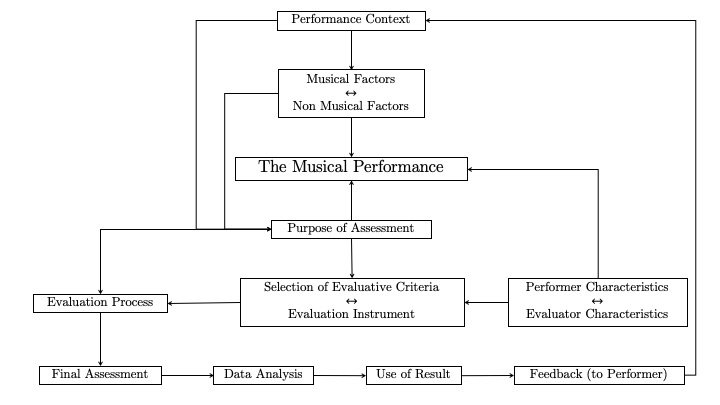
\includegraphics[width=15cm,height=10cm,keepaspectratio]{Assessing}
	\caption{Process Model of Assessing Musical Performance (adapted from \cite{McPhearson1998}))}
	\label{fig:assess}
\end{figure}

McPhearson and Thompson \cite{McPhearson1998} provided a comprehensive summary of the literature regarding the assessment of musical performance, which is depicted in Figure \ref{fig:assess}. To assess "musical performance", various other domains must be considered. Factors such as the "performance context" (e.g., type, purpose, and proportions of the performance) and the "purpose of assessment" (e.g., ranking in competition or research) already influence the evaluation of musical performance. Several musical and non-musical factors can impact the assessment of musical performance. Musical factors, including the choice of repertoire, ensemble size, and expressivity in accordance with the specific composer or period, can affect the rating of a musical performance. Research has demonstrated that non-musical factors, such as the order of appearance, can influence the evaluation of different musical performances \cite{Flores1996}. Listening to various performances of the same piece may result in a greater appreciation of the composition or cause evaluators to begin with higher expectations that gradually adjust to the reality of the performance. Consequently, the characteristics of both the performer and the evaluator are crucial in assessing musical performance. If the performer experiences anxiety or difficulty concentrating during the performance, it significantly impacts the overall quality. Similarly, the personality of the evaluator also plays a significant role. Although research has indicated that training in adjudication does not guarantee better or more consistent evaluation results \cite{Fiske1977}, the evaluator's mood, attitude, and emotional state can influence their assessments. Furthermore, individual listeners' preferences and subjective experiences play a crucial role in the evaluation of musical performance. Musical tastes and preferences vary widely, and what resonates with one listener may not have the same impact on another.  Additionally, the familiarity between the evaluator and performer can substantially impact the evaluation provided. The selection of evaluative criteria is probably the most complex factor for assessing musical performance. To maximise the reliability within the ratings of the evaluators providing a standardised rating scales has proven useful. They establish criteria and guidelines that can be applied uniformly across different performances and context. This constistency allows more reliable comparisons and assessments, enabling performers to track their progress over time. For constructing such scale different criteria are suggested. As first contributor Duerksen provided eight criteria, including rhythmic accuracy, pitch accuracy, tempo, accent, dynamics, tone quality, interpretation, and overall quality \cite{Duerksen1972}. This foundational framework has paved the way for subsequent research. Russell's study devided evaluation criteria into two categories: technical and musical. Technical aspets encompassed tone, intonation, rhythmic accuracy, articulation, and technique, ehile the musical realm involved tempo, dynamics, timbre, interpretaion, and musical expression. Notably, the component of expression had a significant direct effect on the overall perception of quality \cite{Russell2010}. Within institutional frameworkds, the Australian Music Examination Board's Piano syllabus for level 1 underscores accuracy, fluency, rhythmic and metric stability, articulation, dynamics, phrasing, tonal balance, tempo control, and understanding of style and character \cite{AMEB}. The Associated Board of the Royal Schools of Music marking criteria emphasize pitch, time (fluency and rhythm), tone (articulation and dynamics), shape (expressiveness), and overall performance \cite{ABRSM}. Despite the breadth of research and diverse perspectives on performance criteria, a consensus has shown. For evaluation piano beginners' performance the focus lies on technical aspects such as tone and rhythmic accuracy, fluency, articulation, and dynamics, while expressivity complements the components to an overall performance evaulation. \\
In conclusion, the objective rating of musical performance is a complex tast due to the subjectivity of music, the multidimensionality of its elements, the influence of interpretation and artistic choices, contextual considerations, the interplay between technical accuracy and expressive qualities, listener variability, and the limitations of quantitative metrics. While objective measures can provide some insights, a complete evaluation necessitates a balanced approach that incorporates subjective assessments, export judgment, listener feedback, and an appreciation for the artistic an emotional dimensions that make music a captivating and deeply personal form of expression.




\section{Aims/Hypothesis}
musical instrumental prcatice can countervail cognitive and perceptual-motor decline supported by functional and structural brain plasiticity ==> naja, ist nicht mein approach
\\promote healthy mental aging in elderly - independence, autonomy and well-being through musical activities
\chapter{Methods}
\label{cap:Methodology}

\section{Study Design}
For participant recruitment, newspaper articles and posters were created and published in the two study locations (Hanover and Geneva). From various responses, 72 healthy retirees were selected, with 32 from Geneva and 40 from Hanover. All participants were native or fluent in either German or French, depending on the site. The individuals were right-handed and had no more than six months of musical practice throughout their life. None of the participants relied on hearing aids. If they had any current or past neurological diseases, mild cognitive impairments, or early-stage dementia, they were excluded from the experiment. Additionally, none of the participants had any cardiovascular disease, hypertension, obesity, diabetes, or clinical depression.

\minisec{Tests}
Initially, information regarding age, sex, income, and educational level was collected, as shown in Table \ref{tab:demographic}. The income levels were defined on a scale of 1 to 5, indicating the percentage of the national average income: 1 (<25\%), 2 (25-75\%), 3 (75-125\%), 4 (125-175\%), and 5 (>175\%). Similarly, educational levels were scored from 1 to 6: 1 (elementary school), 2 (middle school), 3 (high school), 4 (bachelor's degree), 5 (master's degree), and 6 (PhD).
The participants' cognitive performance was assessed using the Cognitive Telephone Screening Instrument (CogTel). CogTel consists of six subtests that evaluate prospective memory, verbal short-term memory, working memory, verbal fluency, inductive reasoning, and verbal long-term memory. The scores range from 0 (lowest) to 60 (highest) \cite{Kliegel2007}.
Additionally, the participants completed the Cognitive Reserve Index questionnaire (CRIq) to evaluate their cognitive reserve. The CRIq calculates a score based on their educational background, working experience, and the frequency of engaging in various leisure activities such as sports, culture, and travel. An average score is derived from these factors. Scores below 70 indicate a very low cognitive reserve, while scores above 130 indicate a high cognitive reserve \cite{Nucci2012}.
%Furthermore, the participants' subjective assessment of quality of life was measured using the World Health Organization Quality of Life-BREF (WHOQOL-BREF) questionnaire \cite{WHO2012}. This questionnaire assesses four different domains: The physical domain inclues information about pain, sleep, medication use, and mobility. The psychological domain consists of statements about self-esteem, positive and negative feelings, and overall psychological well-being. The social relationships domain focuses on the participants' relationships, social support, and satisfaction with their social interactions. The environment domain assesses the participants' satisfaction with various aspects such as finances, leisure activities, home environment, and access to health services. The scores obtained from the WHOQOL-BREF questionnaire are computed and then transformed to a scale ranging from 0 to 100, with higher scores indicating a better quality of life in each domain. This assessment provides insight into the participants' subjective well-being and their perception of various life domains.

\begin{table}[h]
	\centering
	\caption{Demographic Information of the Sample}
	\label{tab:demographic}
		\renewcommand{\arraystretch}{1.2}
	\vspace{\medskipamount}
	\begin{tabular}{lcc}
		&     &  mean(SD)        \\
		\hline
		Age       &  & 69.6 (3.2) \\
		Education &  & 3.9 (1.4)  \\
		CogTel    &  & 31.0 (7.2) \\
		Income    &  & 2.9 (1.0)  \\
		Site      & Hannover         & 40 (55.6)  \\
		& Geneva         & 32 (44.4)  \\
		Sex      & Male         & 41 (56.9)  \\
		& Female         & 31 (43.1) \\
		CRIq & & 137.4 (15.1)\\
	\end{tabular}
\end{table}
To assess the participants' musical engagement ability, they were required to complete the Goldsmiths Musical Sophistication Index (Gold-MSI) self-report inventory for non-musicians \cite{Mullensiefen2014}. The Gold-MSI consists of six sub-scales that measure different facets of musical sophistication: The Active Engagement evaluates active musical engagement behaviors such as reading about music and the time and money spent on musical activities. The Perceptual Abilities are musical abilities related to perception, such as listening skills. Musical Training measures the extent of musical practice and training. Singing Abilities reflects the skills and activities related to singing. The Emotional Response to Music summarizes the participant's emotional response to music. And the General Musical Sophistication score incorporates various aspects from the other sub-scales to provide an overall measure of musical sophistication.

As Table \ref{tab:goldmsi} shows the scores of the sample is way lower than the norm data provided by the developer but didn't vary as much. The Gold-MSI questionnaire, along with the Cognitive Telephone Screening Instrument (CogTel), was repeated after the intervention.
%relevant?!
\begin{table}[h]
	\centering
	\caption{GoldMSI Scores of the Sample before the Intervention}
	\label{tab:goldmsi}
			\renewcommand{\arraystretch}{1.2}
	\vspace{\medskipamount}
	\begin{tabular}{lcc}
		&    Mean(SD)  & norm(SD)    \\
		\hline
		Active Engagement        & 29.4 (8.3) & 41.52 (10.36)\\
		Perceptual Abilities & 38.7 (9.5)& 50.2 (7.86)\\
		Musical Training    & 10.2 (3.2) &26.52(11.44)\\
		Singing Abilities     & 26.9 (6.5)  &31.67 (8.72)\\
		Emotions         & 22.2 (6.0)  & 34.66 (5.04) \\
		General Musical Sophistication            & 49.3 (12.1) & 81.58 (20.62) \\
	\end{tabular}\par
	\vspace{\medskipamount}
	\textit{The norm data is taken from the large online survey "How Musical Are You?" by BBC LabUK and decribes data from 147,633 adolscent participants \cite{Mullensiefen2013}.}
\end{table}
%Additionally, the participants' musical skills were tested using the Beat Alignment Test (BAT) and the Melodic Discrimination Test (MDT). The BAT assesses an individual's ability to understand or feel a beat and determine if it aligns with the click of a metronome. In a two-alternative-forced-choice task, participants must decide which of two presented beeps is synchronized with the beat \cite{Harrison2018}.
%The MDT evaluates the participant's ability to detect differences in different short melodies. Participants are asked to identify differences in one note among three transposed versions of the same melody \cite{Harrison2017}.
%Furthermore, the participants' scale playing on the piano was tested. They were recorded while playing the following tasks without changing hand position:
%\begin{itemize}
	%\item Slowly playing an up-and-down 5-note scale (C-D-E-F-G) at a pace of 76 beats per minute, with one note played per beat along with a metronome.
	%\item Quickly playing an up-and-down 5-note scale at the same pace, with two notes played per beat along with a metronome.
	%\item Performing the "genie test," where the same note is played five times in crescendo and four times in decrescendo, without following any specific rhythm.
%\end{itemize}
%The recordings of the scale playing were analyzed to calculate the average deviation from the metronome in seconds. A score of 0 would indicate perfect alignment between the participant's playing and the metronome.\\
The participants' motivation to contribute to the study was also assessed by collecting data on their average daily practice time at home. This information was collected at three-month intervals, specifically after three months, six months, and 12 months of the intervention. 
%In the six months after the intervention the participants were asked to note their average pratice time in a music diary.
%To evaluate the participants' recent physical activity, they completed the Physical Activity Scale for the Elderly (PASE). This questionnaire collects information about the type of activity and the duration of activity per day over the past two weeks \cite{Washburn1993}. The PASE questionnaire provides insight into the participants' levels of physical activity during the intervention period.

\begin{table}[t]
	\centering
	\caption{Timeline and Tests}
	\label{tab:time}
	\vspace{\medskipamount}
	\renewcommand{\arraystretch}{1.2}
	\begin{tabular}{lr}
		time	&   activity       \\
		\hline
		t0/0 months of intervention        & %BAT, MDT, Scale,WHOQOL-BREF\\
		\\& CogTel\\
		& GoldMSI\\
		& CRIq\\	 	
		\hline
		3 months of intervention & Ode to joy Simple\\
		& Homework\\
		\hline
		t1/6 months of intervention    		& %BAT, MDT, Scale, WHOQOL-BREF\\
		\\& Homework\\
		\hline
		t2/12 months of intervention    		& %BAT, MDT, Scale, WHOQOL-BREF\\
		\\& CogTel\\
		& GoldMSI\\
		& Ode to joy Simple \\
		& Ode to joy Normal \\
		& Homework\\
	%	\hline
	%	t3/6 months after intervention   & %BAT, MDT, Scale, WHOQOL-BREF\\
	%	\\& Music Diary \\
	\end{tabular}
\end{table}

%The participants' performance on the BAT, MDT, scale playing, WHOQOL-BREF and PASE were measured at specific time points throughout the study: once at the baseline, six months after the intervention started, 12 months after the intervention started and six months after the intervention completion (see Table \ref{tab:time}).
%These repeated measurements allowed for the evaluation of any changes or improvements in musical skills, physical activity levels, and overall cognitive functioning over the course of the intervention.

\minisec{Intervention}
After collecting the baseline data, the intervention began, consisting of one year of piano practice for the participants. The practice sessions were conducted in pairs with piano students as teachers and lasted for one hour per week. The lessons followed a pre-established curriculum (see \ref{cap:Curriculum}).
In the classroom, three Yamaha e-pianos were set up for the participants to use. Additionally, each participant was provided with a Yamaha e-piano to practice at home.
The practice sessions started with imitation and listening exercises, allowing the participants to become familiar with the piano and adopt a relaxed and correct posture. Activities such as clapping, singing, and walking in rhythm were incorporated into the sessions to enhance rhythm and musicality.
Throughout the intervention, the participants gradually learned to read sheet music. A method inspired by  "Piano Prima Vista" by Jens Schlichting (Internote GmbH Musikverlag, 2013) and the Hal Leonard Adult Piano Method was utilized to teach the participants how to read and interpret musical notation.
To reinforce learning and progress, the participants were encouraged to practice for approximately 30 minutes daily at home. They were given exercises and small pieces of music to practice, which they would then present in the following week's session.
Overall, the intervention aimed to provide structured piano practice, guided by piano students, and foster daily practice habits to enhance the participants' musical skills and enjoyment of playing the piano.

\minisec{Assessment of Piano Performance}
To assess the progress of the participants' musical abilities, recordings were made after three and twelve months of piano lessons. After three months, the participants were introduced to a simplified version of Beethoven's "Ode to Joy" (refer to \ref{cap:Ode}) and given a two-week period to familiarize themselves with it. During the recording, the participants were encouraged to play continuously without restarting and to follow the instructions provided on the sheet music, including dynamics and articulation. This recording served as an evaluation of their progress after three months of piano practice.
After twelve months of piano practice, the same version of "Ode to Joy" was recorded again to investigate the long-term effects of the piano lessons. Additionally, the participants learned a new and more challenging version of the same song, which was also recorded. Therefore, each participant had three recordings documenting their progress on the piano (see Figure \ref{fig:rater}).

The progress was evaluated by assessing changes in six variables: articulation, dynamics, rhythm, pitch, fluency, and expressivity over time in the easy version of "Ode to Joy." Possible predictors, such as age, sex, income, education, study location, CRIq score, and CogTel score, were included in the analysis to explain potential changes. The factors of the Goldsmiths Musical Sophistication Index (GoldMSI) were also taken into account. Individual explanatory models were developed for each variable to identify predictors of improvement. Furthermore, it was examined whether the predictors that indicated progress in the musical parameters of the easy version of "Ode to Joy" also predicted better results in the more challenging version of the song. The analysis aimed to identify individual explanatory models for each variable. 

Having analyzed the six musical variables, the possibility of summarizing these variables into a more concise representation of \textit{musicality} was explored. To achieve this, factor analysis was employed, a statistical technique that uncovers underlying latent factors that explain the observed correlations among the variables. By identifying one general \textit{musicality} factor, we aim to capture the essence of participants' musical abilities and provide a comprehensive understanding of how these variables converge to form a cohesive musical aptitude. The generation of a general musicality factor through factor analysis will not only enhance the interpretability of the results but also allow us to draw meaningful conclusions about the participants' overall musical potential. By unifying the six variables into one overarching factor, we can more effectively examine the influence of demographic factors, such as age, gender, and musical training, on this comprehensive measure of musicality.

%\minisec{Progress of Musical Abilities}
%The results of the scale playing, BAT, and MDT were analyzed to assess changes in participants' further musical abilities over time. Similar to the evaluation of piano playing progress, possible predictors were examined and compared to the overall progress in piano playing. By doing so, the analysis aimed to extend the understanding of progress in piano playing to gain insights into the broader development of participants' musical abilities. This analysis would provide a comprehensive understanding of how participants' musical skills evolved over the course of the intervention and help identify factors that influenced their overall musical learning experience.


\section{Evaluation of Piano Performance}
The evaluation of piano recordings was carried out by nine different raters, aged 20-30 ($M=25.78, SD = 3.23$), all with extensive experience in piano playing ($M=18.1, SD = 2.71$ years). Six of the raters held at least a bachelor's degree in music studies, while two had a degree in music education and one a master's degree in psychology. On average, the raters had taught piano for three years. 
The raters were instructed to evaluate the recordings solely based on the given musical parameters. This ensured a more objective assessment and minimized the influence of subjective preferences on the evaluation results. All raters rated the recordings in different randomized orders to reduce possible effects of inattention and dependency on their individual day form.
A scale ranging from 1 to 7 was used by the raters to evaluate six different musical aspects of the the recordings. A rating of 1 represented a very low rating, while 7 indicated a very high rating of the musical parameters. The use of a seven-point scale allowed the raters to discern and evaluate finer nuances and differences in the recordings.
The raters listened to the recordings twice. Both runs consisted of five trials consisting of about 25 excerpts of "Ode to Joy" ($\sim$ 25 min). The raters performed maximally two trials a day with ample time for recovery. The runs were completed in $\sim$ 2 weeks. During the first pass, they focused on articulation, dynamics, and rhythm. The raters assessed the correct execution of indicated articulations in the musical score, such as staccato and legato. They also discerned differences in dynamics, such as forte and piano, as well as crescendos and decrescendos. Rhythmic accuracy was evaluated based on whether the played notes occurred in the correct temporal relationship, disregarding hesitations or interruptions. In the second pass, the raters evaluated fluency, pitch accuracy, and musical expressiveness. Since the subjects were completely new to the piano, fluency was rated very good when the performer could play the piece without interruptions. Pitch accuracy assessed playing only the correct notes. Musical expressiveness was intended to reflect the quality of phrasing and interpretation of the musical piece. 
Prior to each run, raters were trained by the authors by providing them with clear scoring guidelines and examples of low, medium, and high quality musical excerpts. This enabled the raters to judge the recordings based on a common framework, which allowed for comparable scoring. To control the consistency of their ratings, the raters unknowingly evaluated 30 recordings twice. Hence, in total, each rater rated "Ode to Joy" 400 times. 




\section{Statistics}
\minisec{Ratings}
After each rater had submitted all evaluations, the results were statistically analyzed. Aligning the raters' background helped minimize potential differences in their ratings, although characteristic differences remained. These differences was balanced by using the intraclass correlation coefficient (ICC) for each rater. The ICC was initially calculated individually based on the double-rated recordings. It serves as a measure of agreement between the ratings. A correlation of 0 indicates inconsistent ratings, with significantly different evaluations of the same recordings. A correlation of 1, on the other hand, indicates complete agreement in the evaluation of the double-rated recordings. The ICC(3,1) type, according to Shrout and Fleiss \cite{Shrout1979}, was used, employing the two-way mixed effects model with a consistent relationship. The ICC was calculated by subtracting the variance between subjects from the residual variance and dividing the result by the variance between subjects. For the further analysis, the ratings of each rater were weighted by the respective ICC value per variable. 

The use of a larger number of raters with a musical background and the application of an objective rating scale contributed to the objective assessment of the musical parameters of the piano recordings. This approach allows for an informed and comparable evaluation of the musical performance of the subjects and facilitated the development and improvement of their musical abilities.

\begin{figure}[h]
	\centering
	\def \svgwidth{0.9\textwidth}
	\input{Figures/interaction.pdf_tex}
	\caption{Impacts on Musical Performance}
	\label{fig:interaction}
\end{figure}

By minimizing the process model of McPhearson and Thompson \cite{McPhearson1998} through careful disicions, the potential impact on the musical performances were reduced (see Chapter \ref{cap:Background}). This simplification helped lessen the potential impacts on musical performance. We focused on understanding the characteristics of the performance and how they interacted with specific musical or non-musical factors (see Figure \ref{fig:interaction}). This approach could provide more precise insights and enhance the analysis of piano performances.


%2.	 Factor analysis (musikalischer g-Faktor)
%3.	 Improvement over time (individual musical aspects of 1, m-g-Faktor of 2)

\minisec{Modeling Piano Performance}
The data analysis was conducted using a Bayesian mulitilevel model with the R package "brms", developed by Paul Bürkner  \cite{Burkner2017, Burkner2018}. Bayesian statistics are well-suited for accommodating hierarchical models, especially when dealing with data from multiple sources or when there are dependencies among observations. In our study, data were collected from different groups (individuals) and included repeated measures from the same individuals (each rater rated all the participants), making a hierarchical model appropriate for capturing underlying variation and improving estimation accuracy (see Figure \ref{fig:rater}). 

\begin{figure}[h]
	\centering
	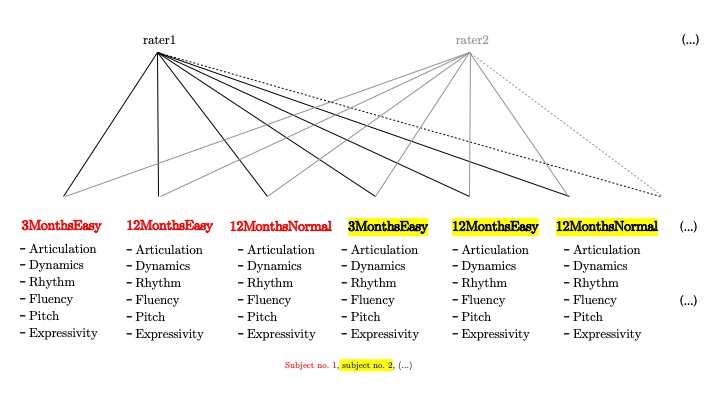
\includegraphics[width=15cm,height=10cm,keepaspectratio]{Rater}
	\caption{Rater System}
	\label{fig:rater}
\end{figure}


Bayesian apporaches have several advantages over frequentist statistics. Unlike frequentist methods that rely on statistical significance and produce dichotomous statements of significance or non-significance, Bayesian analysis provides a posterior distribution that encompasses all plausible values of the effect. Additionally, Bayesian statistics allow for the incorporation of prior knowledge or beliefs about the distribution of the data. 

To analyze results based on a scale ranging from 1 to 7, we utilized Bayesian statistics with a beta distribution, which offers a flexible and intuitive framework for modeling data within a bounded range \cite{Paolino2001}. The beta distribution is characterized by two shape parameters, $\alpha$ and $\beta$. It is well-suited for modeling proportions, probabilities, or continuous variables that are constrained within a finite range, such as a 7-point Likert scale. The versatility of the beta distribution allows it to model various response distributions, including skewed, symmetric, or bimodal distributions, making it applicable to various types of data. By specifying a prior distribution for the beta parameters ($\alpha$ and $\beta$), prior information can be included in the analysis, which can be particularly useful when limited data are available. Bayesian inference provides a framework for quantifying uncertainty in parameter estimation. By combining prior beliefs with observed data, posterior distributions can be obtained, representing a range of plausible values for the parameters. This uncertainty estimation is often valuable when interpreting results and making decisions based on the data. Within this Bayesian framework, we reported 95\% credible intervals (CI), indicating that there is a 95\% probability for the effect to fall within this range. CIs that do not include zero suggest a high likelihood that the effect is either strictly positive or negative, while CIs strongly overlapping with zero indicate a very unlikely effect. For effect sizes that only slighty overlap with zero the Probability of Direction is computed. It serves as an indicator of the existence of an effect and ranges from 50\% to 100\%. It is construed as the probality of a parameter being either strictly positive or negative . The probability of direction can be understood as a parallel to the two-sided p-value. P-values of .1, .05, .01 and .001 correspond approximately to a probability of direction of 95\%, 97.5\%, 99.5\% and 99.95\%. \cite{Makowski2019}. 

For each variable (articulation, dynamics, ryhthm, fluency, pitch, expressivitiy), a Bayesian multilevel approach was employed using the following regression equation. The data were differentiated by the Code, which represents the participants' ID, and different rater effects were considered.
\begin{equation}
	Variable \sim Demographic*time + (1 + time|Code) + (1+ time|rater)
\end{equation}
Prior to analysis, both the variables and the possible demographic predictors were centered at their means and standardized. Here, a one-unit change refers to a change of one standard deviation. Dummy variables (0|1) were used to encode sex (female|male) and site (Hanover|Geneva). Considering that the beta distribution is defined within the interval $(0,1)$, the variables were further scaled down by a  factor of seven, ensuring that the highest conceivable rating correspond to 1 and the lowest to 0. Each outcome variable was analyzed independently with respect to potential demographic predictors. 
The models allowed the slopes and intercepts of the participants to vary for a better model fit. The intercept represents the baseline performance at the beginning of the intervention, while the time effect reveals the change in performance over the study duration. 
Information about model convergence was provided by Rhat values with Rhat < 1.1 indicating satisfactory convergence. To ensure a good fit, posterior predictive checks were performed using the pp\_check function \cite{Gabry2019}.

In conclusion, the statistical apporach involved Bayesian multilevel modeling with a beta family as the response distribution. This approach offered various advantages, including the flexibility to model bounded data, incorporation of prior knowledge, and quantification of uncertainty. The individual analysis of variables allowed for a comprehensive understanding of the effects and predictors of observed changes in musical abilities. 

\minisec{Factor Analysis }
SEM 


A factor analysis was performed to uncover the complex relationships between the different musical variables.
This approach facilitated a deeper understanding of the underlying structure of musical abilities and highlighted the fundamental dimension that underlies the participants' proficiency in various musical aspects. The data used for the analysis was extracted from the calculated models, considering that the values are already weighted by the ICCs of the different raters. 
The number of latent factors was determined through scree plot analysis -- a simple line plot that displays the eigenvalues of the factors in descending order against their corresponding factor numbers. The resulting factor loadings represent the strength and direction of the relationship between the observed variables and the latent factors. Higher absolute values indicate a stronger relationship between the observed variables and the latent factors. To calculate the \textit{musicality} factor for each participant, the factor loadings ($FL_{variable}$) were multiplied by the rated values of the corresponding musical variables and then summed. The resulting composite measure represents the participant's overall \textit{musicality} score, as shown in equation \ref{eq:musicality}.
\begin{equation}
	\label{eq:musicality}
	M = (FL_A \times A) + (FL_D \times D) +\\ (FL_R\times R) + (FL_F\times F) + (FL_P \times P) + (FL_E \times E)
\end{equation}

To assess the development of the potential \textit{musicality} factor, three factor analyses were conducted. One was performed for the baseline and simple version of the "Ode to Joy" ($FA_{0,0}$),  the second after the intervention and the simple version ($FA_{1,0}$), and the third after the intervention with the more challenging version of "Ode to Joy" ($FA_{1,1}$). To avoid complicating and potentially distorting the analysis, the underlying data was extracted using models that only calculated the intercepts of each of the three measuring points. Each analysis resulted in one \textit{musicality} score for each participant at the beginning of the intervention playing the easy version of "Ode to Joy", after the intervention with the easy version, and after the intervention playing the more challenging version of "Ode to Joy". 

Subsequently, Bayesian multilevel models were established to explore potential demographic predictors. As the raters are already weighted in the input data and the input data are the estimate intercepts of all participants, the regression equation follows the simple struture shown in equation \ref{eq:musdem}:
\begin{equation}
	\label{eq:musdem}
	Musicality \sim Demographic * time
\end{equation}
Given that the data is not limited to specific values, the outcomes are modeled following a normal distribution.
\chapter{Results}
\label{cap:Results}
The evaluation of the piano recordings yielded promising results, offering valuable insights into the reliability and consistency of the rater system. The slopes and intercepts of the piano progress varied strongly among the participants, which is expected given their diverse individual backgrounds. The results are categorized into four main areas of evaluation: the rater system, the progress of piano playing, the progress in other musical abilities, and the exploration of a potential general \textit{musicality} factor.


\section{Rater System}

With the double rated evaluations the Intraclass Correlation Coefficient (ICC) values were computed to determine the level of agreement and consistency among the raters' evaluations. Table \ref{fig:icc} presents the ICC values for each rater across the six variables.

\begin{figure}[h]
	\centering
	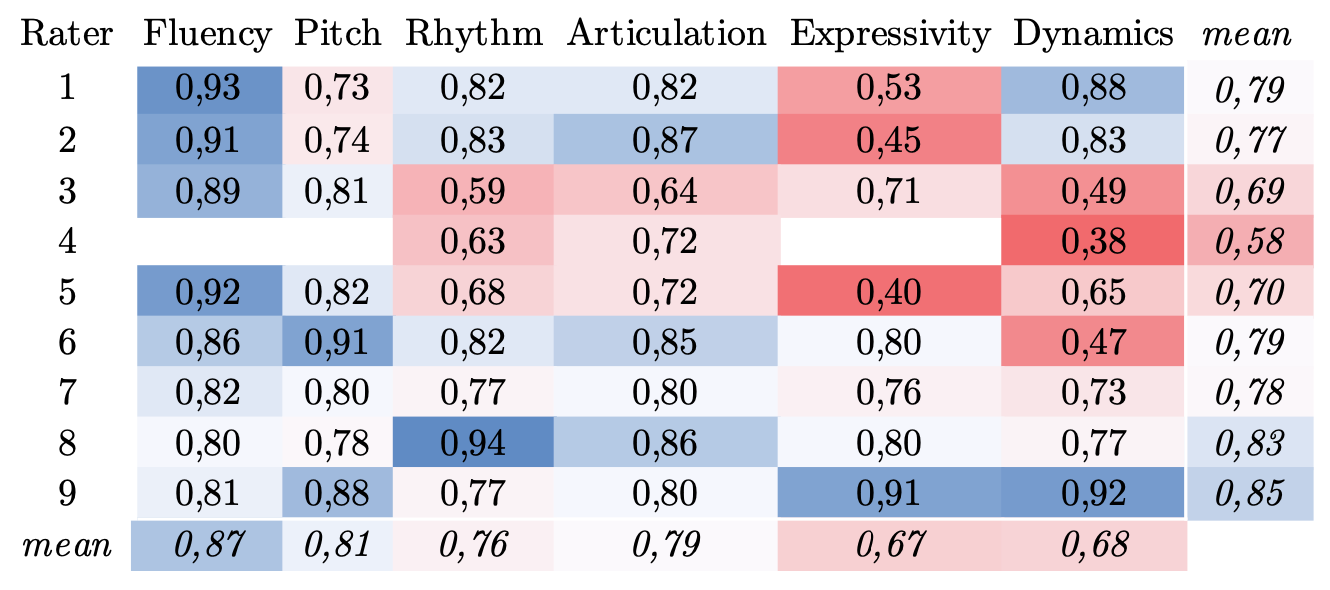
\includegraphics[width=12cm,height=10cm,keepaspectratio]{ICC}
	\caption{ICC Values of Each Rater for Each Variable}
	\label{fig:icc}
	\textcolor{blue}{> .9; excellent}, \textcolor{lightblue}{.75 - .9; good }, \textcolor{red}{.5 - .75; moderate }, \textcolor{purple}{> .5; poor reliability} \cite{Koo2016}.
\end{figure}

The ICC values indicated varying degrees of agreement among the raters for each variable. For fluency, the ICC values ranged from 0.803 to 0.931, indicating a high level of consistency among the raters' assessments. Similarly, pitch exhibited strong agreement among the raters, with ICC values ranging from 0.733 to 0.91. Rhythm evaluations also demonstrated a high level of agreement, with ICC values ranging from 0.586 to 0.943. Articulation was assessed with moderate to high reliability, as indicated by ICC values ranging from 0.64 to 0.858. Expressivity showed moderate agreement among the raters, with ICC values ranging from 0.404 to 0.907. The evaluations of dynamics exhibited the greatest variability among the raters, with ICC values ranging from 0.378 to 0.915. Overall, the results suggest that the raters demonstrated good to strong consistency in evaluating fluency, pitch, rhythm, and articulation. However, there was more variability in the assessments of expressivity and dynamics.

The ICC values reveal considerable variability in consistency among the raters. For instance, Rater 8 and Rater 9 demonstrate higher reliability compared to Rater 3 and Rater 4. Despite analyzing factors such as age, years of piano practice or teaching, no clear explanations for these differences were found, likely due to the small group size and alignment of raters in these factors. Furthermore, no differences were observed between different university degrees, such as music educators and musicians, in terms of rating.
In the subsequent analysis, the ratings were weighted based on the ICC values per rater and variable. This approach ensured that raters with higher consistency had a greater impact on the analysis of musical performance compared to raters with lower ICC values.

The Interrater correlation also showed moderate to high reliability among all raters (see figure \ref{fig:heat}). Among the raters no outlier could be found. As shown in table \ref{tab:interrater} the correlation coefficients are between 0.78 and 0.93. Expressivity shows the lowest reliability of 0.78, still being in a good range. The raters agreed most on fluency as shown by the correlation score of 0.93. Articulation and Pitch follows directly. 
\begin{table}[h]
	\centering
	\caption{Interrater Coefficients for Each Variable }
	\label{tab:interrater}
	\renewcommand{\arraystretch}{1.2}
	\vspace{\medskipamount}
	\begin{tabular}{l|cccccc}
		&    Articulation	& Dynamics & Rhythm & Fluency & Pitch & Expressivity     \\
		\hline
		Interrater Coefficient       &  0.92 & 0.87 & 0.87 & 0.90 & 0.93 & 0.78\\
	\end{tabular}\par
	\vspace{\medskipamount}
\end{table}

\section{Piano Progress}
\label{cap:PianoProgress}

neues, richtiges bild!

\begin{figure}[h]
	\centering
	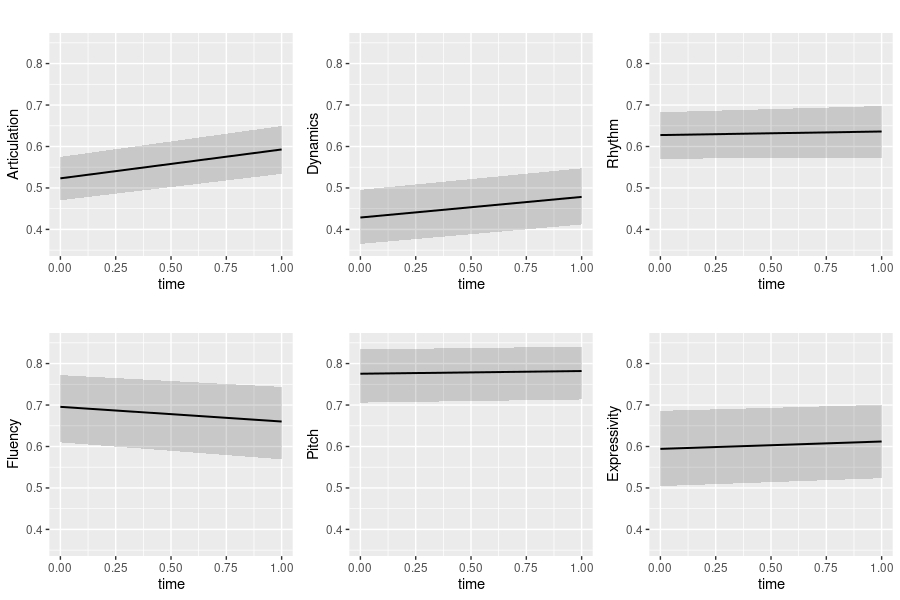
\includegraphics[width=15cm,height=10cm,keepaspectratio]{pred_vals}
	\caption{Predicted Values over time}
	\label{fig:PredVals}
\end{figure}

The models convergered with a Rhat-value of 1.0, indicating a satisfactory convergence of the Markov Chain Monte Carlo algorithm used for estimation. The analysis of piano playing progress across the six variables articulation, dynamics, rhythm, fluency, pitch, and expressivity, revealed generally strong variations in slopes and intercepts. Examining the changes in these variables over time, various patterns emerged (see Figure \ref{fig:PredVals}). Notably, while articulation showed the strongest improvement, the score for fluency decreased. Below, a detailed analysis of each variable is presented. 

\minisec{Articulation}
 The intercept for articulation is 0.52 (95\% CI [0.47, 0.59]), indicating a moderate level of articulation proficiency at the beginning. Over time, there was a clear positive time effect (0.43, [0.18, 0.68]), suggesting that participants' articulation skills improved during the intervention. On average, the subjects displayed a 10,6\% improvement in articulation as a result of the intervention, starting from 49.6\% improving to 60.2\%.
Although the effect values for demographic factors are relatively small, trends can be observed in relation to articulation scores. Participants with higher income (0.23, [0.02, 0.43]) displayed higher articulation scores initially. Similarly, participants with higher cognitive reserve (0.10, [-0.11, 0.30]), higher educatioin (0.15, [-0.05, 0.35]) and higher CogTel scores (0.13, [-0.07, 0.33]) exhibited higher articulation scores initially. Although the 95\% CI of cognitive reserve, education and CogTel include zero, the variables have a 82\%, 93\% and 90\% probability of positively affecting musical performance. The goldMSI categories showed no effect on participants' initial articulation performance. 
To understand if the effect of demographic factors on articulation changed over time, we examined the interaction between each demographic factor and time. Participants who spent more time on their homework were 93\% more likely to show improvement over time (0.18, [-0.06, 0.41]). It is 97\% likely that younger participants also improved more (-0.20, [-0.41, 0.01]).
Participants with self-reported lower levels of musical engagement improved more in articulation scores during the intervention (-0.29, [-0.51, -0.08]). The effect of emotions towards music and singing abilites on articulation over time was also clearly negative (-0.23, [-0.44, -0.02]; -0.28, [-0.45, -0.05]). Perceptual abilities (-0.1, [-0.31, 0.11]) and musical training (-0.12, [-0.33, 0.10]) had a negative effect on articulation during the intervention, both being 85\% likely to be negative. Participants with lower scores in these areas showed more increases in articulation compared to those with higher scores. General sophistication had a negative effect on articulation over time (-0.19, [-0.34, -0.05]). Participants with higher levels of general sophistication displayed a decrease in articulation scores during the intervention.
After twelve months of intervention, participants with higher CogTel (0.15, [-0.03, 0.39]) and higher income (0.21, [-0.03, 0.45])  were 90\% and  96\% likely to have higher articulation scores on the more difficult version of "Ode to Joy". Additionally, homework was 95\% likely to have a positive impact (0.21, [-0.04, 0.47]).

\minisec{Dynamics}
The intercept for piano performance in terms of dynamic quality is 0.44 ([0.38, 0.52]), indicating a relatively low baseline performance. However, the time effect of 0.38 ([0.08, 0.67]) suggests a positive development over time, indicating that participants showed improvement in dynamics during the intervention. On average, the participants' dynamic skill improved by 8.9\% over the course of the intervention, from  39.6\% to 48.5\%. 
Initially, education had an impact on the dynamic scores. Participants with higher education scored generally better in the easy version of "Ode to Joy" in the first measurement (0.19 [0.00, 0.38]). In addition, participants from Geneva were likely to have better dynamic quality (0.13, [-0.07, 0.32]), with a 90\% probability of the effect values being positive. Participants who self-reported having a high score regarding their emotions towards music scored clearly better than the others (0.24, [0.04, 0.42]).
Over time, the younger participants were 95\% likely to improved more (-0.22, [-0.47, 0.04]). Participants with more cognitive reserve seemed to show greater improvements (0.17, [-0.09, 0.43]), but the effect was not very credible (91\% of all effect values are positive). Again, participants with less musical emotion improved more (-0.37, [-0.61, -0.13]). A negative trend (95\% of effect values were negative) was observed regarding participants with low musical engagement, as they showed more improvement than others. 
In the more difficult version of "Ode to Joy", participants with higher cognitive reserve scores performed better (0.28, [0.06, 0.50]). Furthermore, female participants were 90\% and participants with higher CogTel scores 93\% likely to reach higher dynamic skills. 

\minisec{Rhythm}
The intercept for rhythmic skills is 0.63 [0.52, 0.70], indicating a moderate baseline performance compared to other variables. Rhythmic skills did not change over time (-0.01, [-0.16, 0.28]).
Regarding demographic factors, the analysis revealed that men exhibited higher rhythmic skills at the beginning (0.25,  [0.01, 0.49]). Additionally, participants with higher income (0.19, [-0.02, 0.39]), higher CogTel scores (0.20, [-0.01, 0.40]), less age (-0.16, [-0.35, 0.05]), and higher musical engagement (0.12, [-0.08, 0.31]) were most likely to show higher rhythmic scores. Cognitive reserve also had a positive effect on rhythmic skills (0.38, [0.14, 0.61]).
Over time, lower educated participants were 90\% sure to improve more (-0.13,[-0.32, 0.07]). Participants with lower income (-0.15, [-0.36, 0.05]) and lower CogTel scores (-0.15, [-0.35, 0.05]) were 93\% likely to improve more. Emotions towards music were 90\% likely to have a negative effect (-0.13, [-0.33, 0.07]), suggesting an increase in rhythmic skills over time for participants with less emotions. 
At difficulty level 1, participants with higher cognitive reserve were associated with better rhythmic scores (0.20, [-0.01, 0.42]), as well as higher perceptual abilities (0.22, [0.02, 0.43]), and general sophistication (0.17, [-0.05, 0.38]).

\minisec{Fluency}
The intercept for fluency is 0.71 [0.62, 0.78], indicating a relatively high baseline performance. However, there is a  likely negative time effect of -0.09 [-0.32, 0.14], suggesting a negative trend over 2.4\% in fluency over the intervention period.
Regarding demographic factors, being male had a positive effect (0.25, [0.01, 0.49]). Participants from Hanover also had higher fluency scores (-0.18, [-0.43, 0.07]), with a 92\% probability of being real. Higher cognitive reserve had a strong positive effect on fluency (0.38, [0.14, 0.61]), and no effect was observed for goldMSI categories.
While musical training had a possible but small positive effect on fluency over time (0.13, [-0.07, 0.33]), emotions had a possible but negative effect on fluency over time (-0.18, [-0.38, 0.02]), being 90\% and 96\% likely to be positive or negative, respectivly.
At difficulty level 1, being male had a 92\% likely positive effect on fluency (0.14, [-0.15, 0.45]). Participants with higher cognitive reserve were rated to play more fluent (0.32, [0.01, 0.62]) and again participants from Hanover scored higher (0.12, [-0.08, 0.33]), with the effect being 92\% likely to be positive. Higher perceptual abilities (0.28, [-0.01, 0.57]) and higher general musical sophistication (0.20, [-0.10, 0.51]) showed postive effects being 97\% and 91\% likely on fluency. 


\minisec{Pitch}
The analysis of pitch data revealed a high baseline performance, with an intercept of 0.78 [0.71, 0.84]. Participants demonstrated a high starting level of pitch accuracy. Over the intervention period, there was no a trend of positive improvement in pitch (0.16, [-0.14, 0.46]).
At baseline, CogTel and cognitive reserve had positive effects on pitch, with coefficients of 0.23 [0.00, 0.47] and 0.27 [0.05, 0.50], respectively.
Participants with lower CogTel scores 90\% likely improved more (-0.13, [-0.33, 0.08]). Cognitive reserve showed a negative effect, indicating that participants with higher cognitive reserve demonstrated less improvement in pitch accuracy (-0.28, [-0.56, -0.00]). Similarly, musical engagement was associated with reduced pitch improvement (-0.26, [-0.54, -0.03]). Singing abilities (-0.21, [-0.50, 0.08]) also had a 92\% likely negative effect on pitch improvement. Moreover, emotions towards music showed a strong negative effect on pitch improvement (-0.37, [-0.65, -0.10]). 
At difficulty level 1, age showed a 95\% likely negative effect (-0.21, [-0.45, 0.03]), indicating that younger participants achieved higher pitch scores. Cognitive reserve had a positive effect, with an effect size of 0.26 [0.02, 0.51], indicating that participants with higher cognitive reserve scores performed better on pitch evaluation. Also participants from Hanover were 94\% to score higher pitch scores (-0.19, [-0.43, 0.05]).

\minisec{Expressivity}
The analysis of expressivity data revealed a moderate baseline performance, with an intercept of 0.61 [0.52, 0.71]. Over the intervention period, there was a small likely improvement in expressivity, as evidenced by a time effect of 0.15 [-0.05, 0.34].
Higher education and higher CogTel scores had a small positive with a probability of 91\% influence on expressivity skills after three months (both 0.12, [-0.06, 0.3]). Cognitive reserve was 97\% likely to have a positive impact (0.16, [-0.01, 0.33]).
The time spent on homework had a clear positive effect on the development of expressivity performance (0.21, [0.04, 0.39]).
Participants with lower emotion towards music demonstrated 94\% likely better expressiveness (-0.13, [-0.30, 0.03]).
Additionally, higher cognitive reserve showed a strong positive effect on expressivity at the more challenging version of "Ode to Joy" (0.25, [0.05, 0.45]), indicating that participants with more cogntive reserve sophistication performed better in expressivity. Also men were 91\% likely to score higher on expressivity (0.14, [-0.07, 0.34]). Partcipants with higher perceptual abilities reached higher expressivity scores in the more challenging version after 12 months (0.24, [0.05, 0.44]). Similarly, participants with higher general sophistication were 94\% likely to score higher (0.17, [-0.04, 0.38]).


%in discussion?
Conclusively, the participants made clear improvements in articulation and very likely improvements in dynamics, whereas pitch, expressivity, and rhythm did not change over time. Moreover, fluency likely decreased over time. For and overview of the coefficents of all predictors impacting piano performance at different levels of difficulty, see Table \ref{tab:preds}. Only a few demographics could be confirmed to potentially predict the performance in various piano-related skills. Overall, it could be suggested that younger people with more cogntive reserve and a higher CogTel achieve higher scores in different aspects of piano performance. While people who describe themselves to have more emotions toward music, more singing and perceptual abilities, and a higher general musical sophistication reach higher scores when performance is tested, those who have less of all improve better over time. To generalize these observations the analysis is repeated on a potential \textit{musicality} factor which could be extracted through factor analysis. 

\section{One General \textit{Musicality} Factor}

faktorenanalyse mit sem path and predictors?


Three separate factor analyses were conducted revealing patterns of shared variance that contribute to participants' overall musical performance: one at the baseline with the easy version of "Ode to Joy" ($FA_{0,0}$), another after 12 months of intervention with the easy version ($FA_{1,0}$), and the third after the intervention with the more challenging version of "Ode to Joy" ($FA_{1,1}$).
\begin{figure}[h]
	\centering
	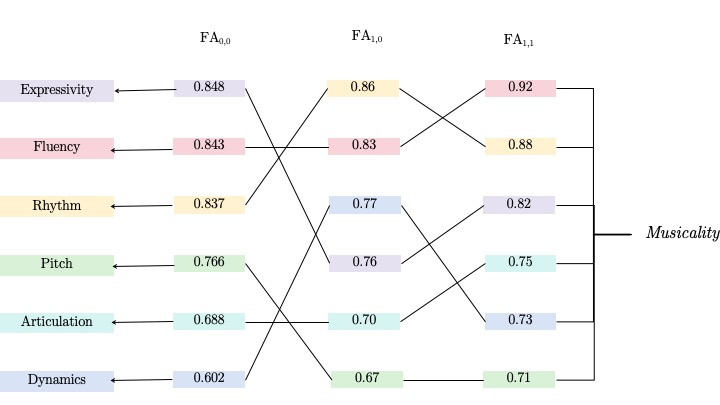
\includegraphics[width=15cm,height=10cm,keepaspectratio]{Loadings}
	\caption{Factor Loadings on \textit{Musicality}}
	\label{fig:loadings}
\end{figure}

Results from all three factor analyses consistently indicated the presence of only one dominant factor, which was labeled as \textit{musicality}. This single latent factor accounted for 59\% of the total variance in the data for both $FA_{0,0}$ and $FA_{1,0}$, and 65\% of the total variance in $FA_{1,1}$. The observed musical variables (articulation, dynamics, rhythm, fluency, pitch, expressivity) all showed positive and moderate to strong factor loadings ranging from 0.60 to 0.85 in $FA_{0,0}$, from 0.67 to 0.86 in $FA_{1,0}$, and from 0.71 to 0.92 in $FA_{1,1}$ (see Figure \ref{fig:loadings}). These factor loadings indicated a robust positive relationship between each musical variable and the underlying \textit{musicality} factor, suggesting that each variable contributed substantially to participants' overall musical performance. 

Regarding changes in the musical variables over time (see \ref{cap:PianoProgress}), the calculated participants' \textit{musicality} scores (see \ref{eq:musicality}) showed stability throughout the intervention and difficulty levels. Notably, a considerable increase in the stability of one \textit{musicality} factor was observed after the intervention with the challenging version of "Ode to Joy" ($FA_{1,1}$). The measures of fit, such as RMSEA index and Tucker Lewis Index of factoring reliability, indicated that all three factor analyses provided a goof fit to the data. The highest Tucker Lewis Index of factoring reliability was observed in $FA_{1,1}$.

After extracting the \textit{musicality} factor, the factor loadings were multiplied with the original data and summed up to calculate a \textit{musicality} score for each participant. These \textit{musicality} scores ranged from -0.8 to 6.5, with higher values indicating a higher level of overall musical abilities and lower values suggesting a lower proficiency in multiple musical aspects. Subsequently, the \textit{musicality} scores were analyed to investigate potential impacts of demographic factors. 
At the beginning of the intervention, the intercept for \textit{musicality} was estimated at 2.9 with a 95\% CI  of [2.81, 2.99], representing the average \textit{musicality} score for participants. A clear time effect was observed, indicating that participants' \textit{musicality} scores decreased by approximately 0.37 units [-0.49, -0.24] from the beginning to after the intervention with the easy version of "Ode to Joy" (see Figure \ref{fig:mus}).
\begin{figure}[h]
	\centering
	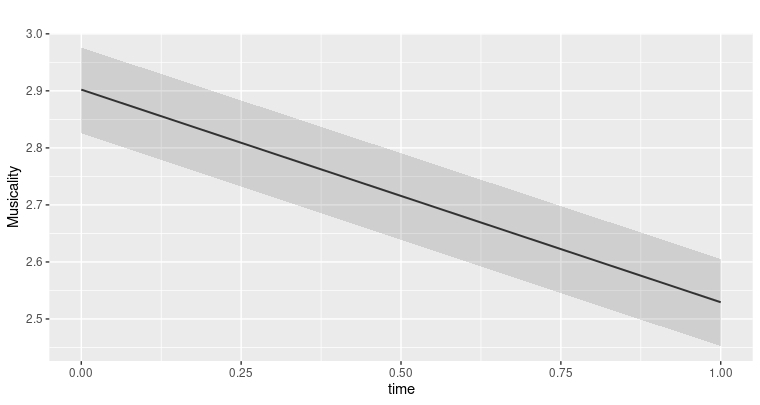
\includegraphics[width=15cm,height=10cm,keepaspectratio]{Musicality}
	\caption{Predicted Values of \textit{Musicality} over time}
	\label{fig:mus}
\end{figure}

The results further revealed only a few demographic predictors that influenced participants' \textit{musicality} scores. Initially, younger participants scored slightly higher in \textit{musicality} (-0.08, [-0.18, 0.01]). Partcipants with higher cognitive reserve scores achieved better overall scores (0.10, [0.01, 0.19]). Aditionally, participants with higher CogTel scores obtained higher \textit{musicality} scores (0.08, [0.00, 0.18]). The effect sizes are small but clear.
Over time, participants with more cognitive reserve and higher CogTel scores showed less decrease in \textit{musicality} scores (cogntive reserve: 0.19, [0.06, 0.32]; CogTel: 0.19, [0.07, 0.32]). Similarly, the scores of younger (-0.22, [-0.35, -0.09]) and male (0.2, [0.09, 0.32]) participants diminished less. Participants with higher income and those who spent more time on their homework also experienced a smaller decrease in \textit{musicality} scores (income: 0.16, [0.03, 0.29]; homework: 0.34, [0.21, 0.47]). Moreover, participants who were less engaged in musical activities and had fewer emotions towards music demonstrated a lower decrease of \textit{musicality} scores after the intervention with the easy version of "Ode to Joy" (Musical Engagement: -0.25, [-0.38, -0.11]; Emotions: -0.37 [-0.49, -0.24]). Better singing abilities and more general sophistication in music also minimized the decrease of \textit{musicality} over time (Singing abilities: -0.25, [-0.38, -0.12]; general sophistication: -0.18, [-0.31, -0.05]). 
In the more challenging version of "Ode to Joy", participants with higher education (0.2, [0.06, 0.34]), higher perceptual abilities (0.36, [0.22, 0.5]), higher CogTel scores (0.26, [0.11,0.4]) and more cognitive reserve (0.47, [0.33, 0.61]) performed better compared to other participants. Participants from Hannover (-0.31, [-0.45, -0.17]) and those who spent more time doing homework (0.23, [0.08, 0.28]) had a positive impact on musical performance. Additionally, better singing abilities and greater general sophistication in music also positively influenced \textit{musicality} scores after the intervention with the challenging version of "Ode to Joy" (0.19, [0.05, 0.34]; 0.26, [0.12, 0.41]).



%\section{?? Progress of Musical Abilities}
%\subsection{BAT, MDT, Scales}
%\subsection{GoldMSI}


\chapter{Discussion}
\label{cha:Discussion}

%development of specific domains

The findings offer valuable insights into the development of motor skills,  particulary piano playing skills, among older individuals. The notion that older people can still develop motor skill could be supported through the context of piano performance. 
Specifically, the study unveiled positive advancements in the domaincs of articulation and dynamics. These improvements are intriguing as they encompass techinical factes often associated with precision and control (TRUE OR NOT?). The increase in expressivity, although subtle, also aligns with these developments, as expressivity is often contingent on effective articulation and dynmaics. However, it is intriguing to note that rhythm did not show a similar level of positive development. This discrepancy needs further investigation and might be explained by the multifaceted nature of rhythm perception and production, which potentially involves cognitive factors that interact differently with aging.
In contrast, the participants' piano playing fluency showed a negative trend over the year of practice. It is worth considering the methodological aspect of this finding. After 12 months, participants were recorded playing both versions of "Ode to Joy". While one version was more difficult than the other, both versions contained the same song, differing only in small nuances. That could have led to confusion between the versions and potentially resulted in poorer performance on the easier version than after three months. Similar logic could apply to the pitch consistency. Further studies should carefully select musical pieces for observation and ensure clearer differentiation more among them. 
The variations in developmental trajectories across the different domains underscore the complexity of the acquistion of musical skill. Each domain seems to require unique cognitive, sensory, and motor demands, that should be further looked into.



Expressivitiy on midi keyboards - musically speaking.....//
noch längere studie
langzeit?
%auswahlprozess? variablen wahl, skala 1 bis 7 wahl, 


%predicted development
%%Musical development was difficult to predict, with some demographic variables influencing only some musical aspects.

The prediction of musical development proved to be challenging, with certain demographic variables influenciny only specific aspect of musical skill. This suggests that musical development is a multifaceted process influenced by many factors, including individual characteristics, history, and perhaps cognitive or physiological changes associated with agig.

%musicality factor
%%factor analysis indicated a one factor solution, which we call musical g-factor.
The factor analysis allowed us to reduce the dimensionality of the data and summarize the information from the six individual musical variables into a single composite measure. This approach provides a more parsimonious representation of musical abilities and enables a deeper understanding of the underlying construct. The analysis yieled a noteworthy result -- a single factor solution, we termed musical g-factor \cite{Pausch2022}. The factor loadings suggest that \textit{musicality} is a multdimensional construct, incorporationg various aspects of musical abilties. The presence of this overarching factor suggests the interconnectivty of musical skills. The identification of this musical g-factor has implications for the understanding of musical skill development. It suggests that while skills may be domain-specific in nature, they are still governed by a common cognitive substrate linked to musical aptitude. This also highlights the potential for transfer of skills across different domains, where improvements in one domain might positively influence another due to the shared musical g-factor.
The multidimensional nature of \textit{musicality} underscores the importance of developing well-rounded musical skills, encompassing articulation, dynamics, rhythm, fluency, pitch, and expressivity. Music educators may benefit from integrating diverse exercises and activities that target these specific musical dimensions to foster overall musical growth in their students.



Rater system \\

%Inter Rater Variability:

Inter-rater reliability, or the extent to which raters disagree in their assessments, is a crucial aspect of any rating system. In our study, the inter-rater reliability exhibited notable patterns across the different variables. Articulation, pitch, and fluency displayed a higher level of consistency among raters, with inter-rater reliability coefficients exceeding 0.9. Expressivity, dynamics, and rhythm demonstrated a slightly lower but still substantial inter-rater consistency, with coefficients hovering around 0.8.
The reasons behind these variations in consistency could be attributed to the inherent characteristics of each variable. Articulation, pitch, and fluency might be easier for raters to consistently grasp due to their more concrete and quantifiable nature. These elements could be objectively identified and evaluated, leading to fewer discrepancies in interpretation among raters. On the other hand, dimensions like expressivity, dynamics, and rhythm may involve more subjectivity, allowing room for differing perceptions and preferences.
Despite these variations, the inter-rater reliability across the panel remained generally high. The raters exhibited consistent evaluations, and the overall consensus on the recordings was evident. This reinforces the notion that even with differences in interpretation, a rater system can yield reliable outcomes.

%Intra Rater Variability:

Intra-rater reliability refers to the agreement of a single rater's assessments across multiple instances. Our analysis revealed that intra-rater reliability was also influenced by the specific evaluation dimensions. Articulation, pitch, rhythm, and fluency displayed higher levels of agreement within raters, whereas dynamics and expressivity exhibited more fluctuation.
The differences in intra-rater reliability can again be indicative of the complexity and subjectivity associated with certain dimensions. The more concrete variables might be easier for raters to consistently assess, while those involving personal interpretation or emotional resonance may lead to varying responses over time.
Notably, the ICCs indicated moderate to good levels of agreement in the ratings, with some reaching excellent levels. This suggests that the raters maintained a certain level of agreement in their assessments over multiple rounds of evaluation. The variation in ICCs did not depend on educational background or teaching experience. 
Future research could delve deeper into understanding the factors influencing individual raters' tendencies towards agreement or variability. Investigating the correlation between personal traits, background, and the specific dimensions that showed varying levels of reliability could provide valuable insights into the rater's decision-making process.

In conclusion, the rater system demonstrated a satisfactory level of inter-rater and intra-rater reliability. The findings highlight the importance of considering intra- and inter-rater reliability in the evaluation of piano recordings. The consistent assessments of fluency, pitch, rhythm, and articulation suggest that these musical parameters can be considered to be evaluated robust and reliable. However, the variability observed in the evaluations of expressivity and dynamics indicates potential differences in the interpretation and perception of these aspects among the raters and needs further investigation to explore the factors contributing to the variability in evaluations of expressivity and dynamics. The variations observed shed light on the complex interplay between the nature of the evaluated dimensions, and rater subjectivity. 
These findings underscore the significance of well-defined evaluation criteria, continuous communication, and suggest an accurate investigation of the raters' personality and background for achieving reliable and comprehensive assessments.



%raus? Careful decisions were made to evaluate the piano performances, following the model described in chapter \ref*{cap:musicalabilities}, in order to minimize possible sources of friction. The performance context and assessment's purpose were clear and unchanged throughout ratings, allowing for the exclusion of these factors from the analysis. 



\chapter{Summary and Outlook}
\label{cap:Summary}

%\input{Chapters/QandA}
%\input{Chapters/LoremIpsum}

%-----------------------------------------------------------------------------
% Bibliography
%-----------------------------------------------------------------------------
\cleardoublepage
\refstepcounter{Hilfszaehler}
\addcontentsline{toc}{chapter}{\bibname}
\protect\bibliographystyle{unsrtdin} % This style is not mandatory. Another would be e.g. natdin.
\bibliography{Masterarbeit}



%-----------------------------------------------------------------------------
% Appendix		 	     
%-----------------------------------------------------------------------------
\cleardoublepage
\FloatBarrier	% Prevents figures/tables to move to appendix
\addtocontents{toc}{\protect\setcounter{tocdepth}{2}}
%Prevents Appendix sections to show in the TOC if you set the number to 0

\captionsetup{list=no}	
% Prevents captions of figures/tables in appendix t appear in the list of figures and tables

\begin{appendix}
\newpage\thispagestyle{empty}~
\vfill{}\vspace{-1\parskip}
\begin{center}\textsf{\textbf{\huge \appendixName}}\end{center}{\huge \par}
\vfill{}
~
%TODO	%%% ADD YOUR APPENDIX CHAPTERS HERE %%%
\newpage
\chapter{Appendix}
\label{cap:Appendix}
\section{Ode to Joy Sheets}
\label{cap:Ode}
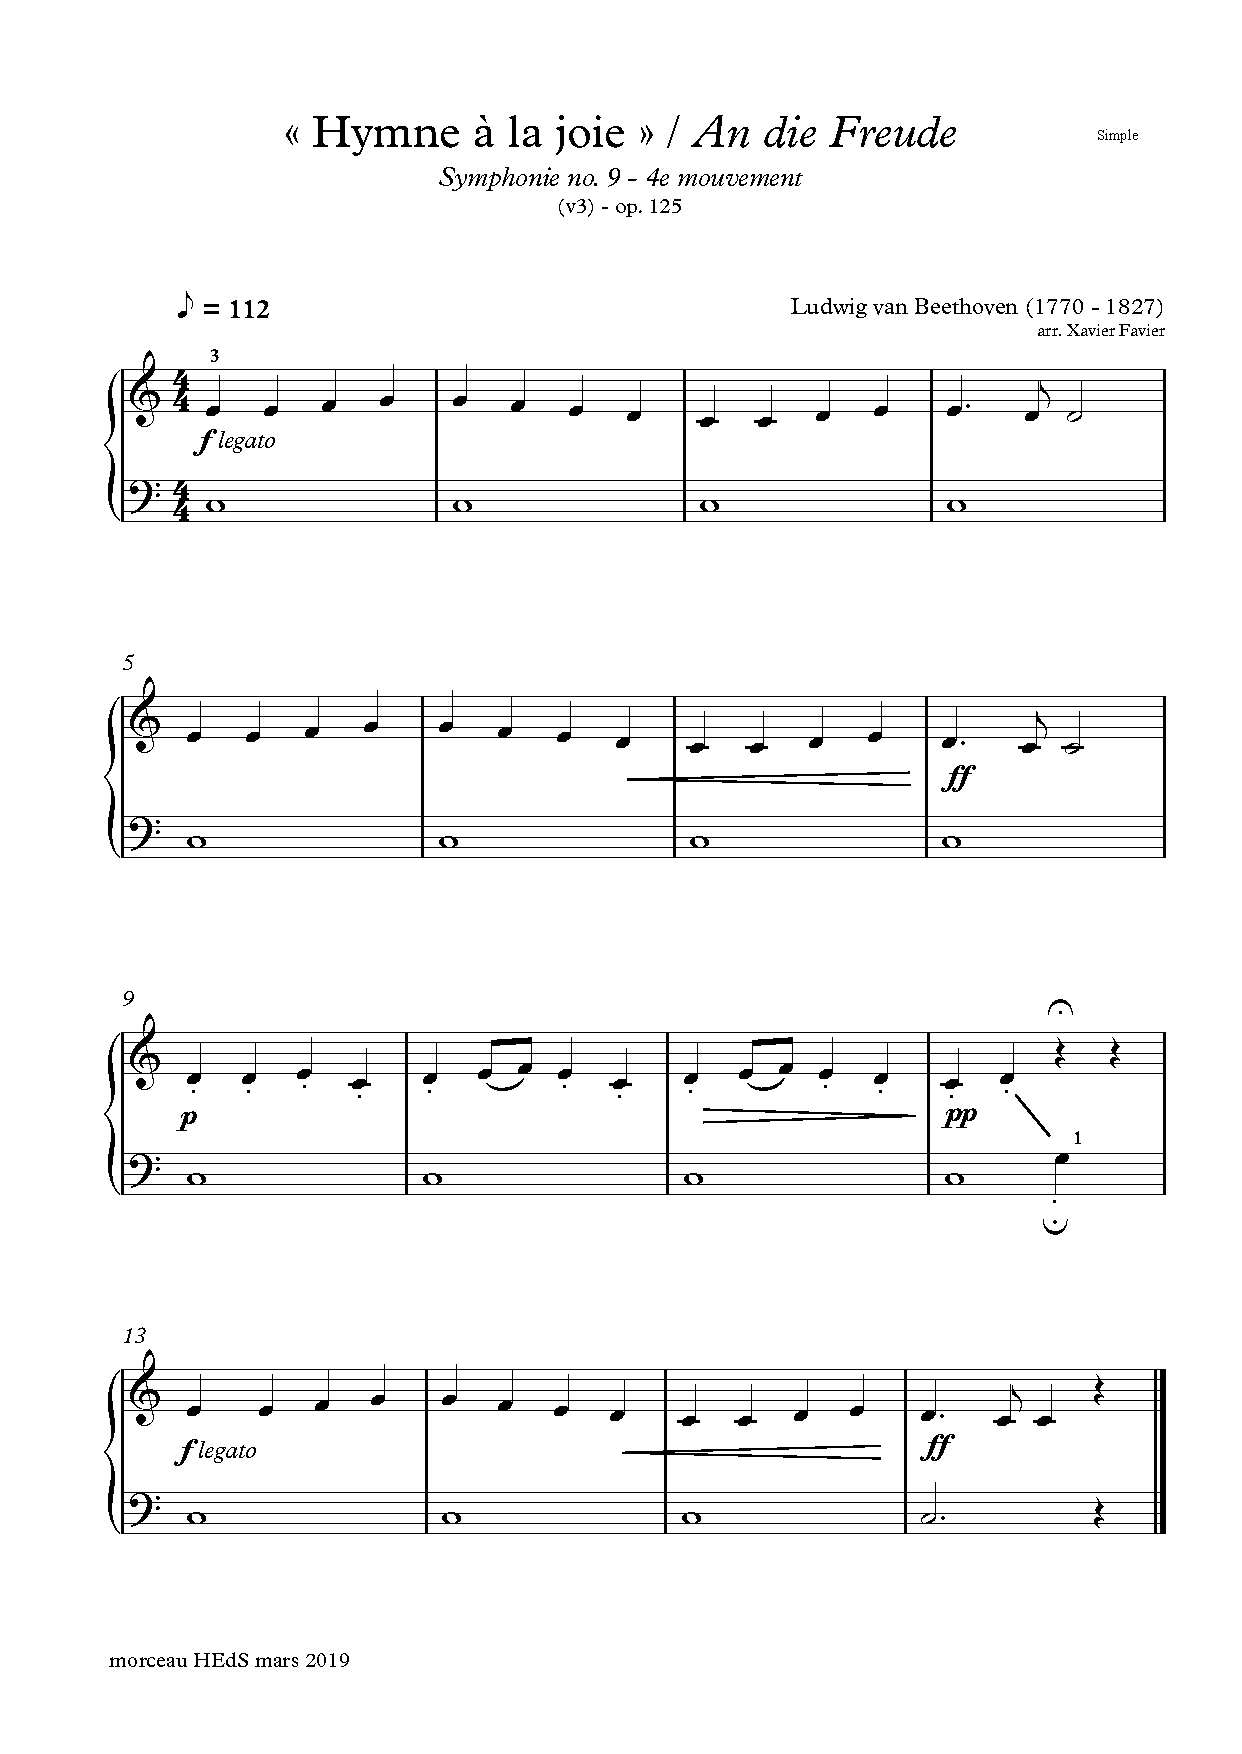
\includepdf{BeethovenOdeSimple.pdf}
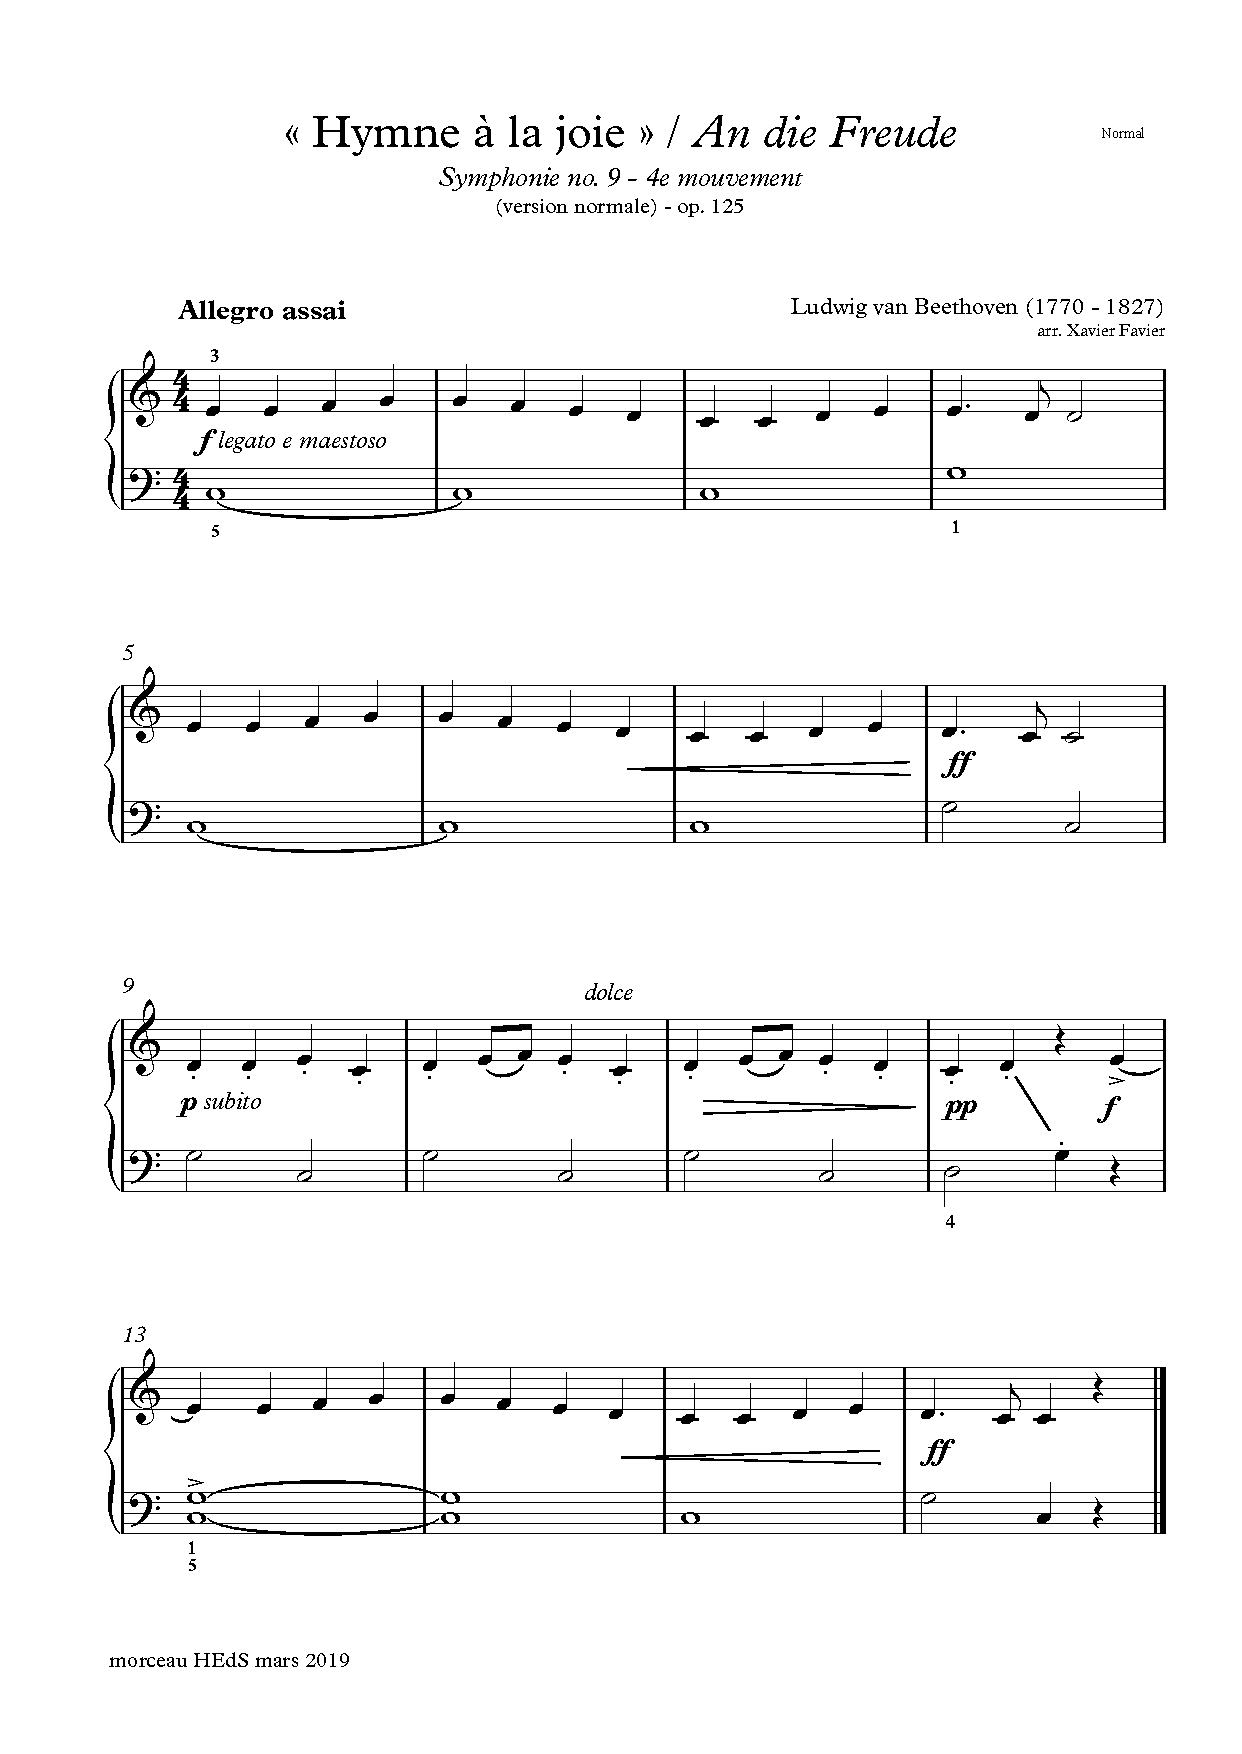
\includepdf{BeethovenOdeNormal.pdf}
\section{First Six Months Curriculum for Playing Piano}
\label{cap:Curriculum}
Each participant received an electronic piano, adjustable stool, and headphones for homework\footnote{Yamaha Germany \& Yamaha Switzerland generously offered the electronic pianos (Yamaha P-45 B)}.
	
Courses: In the beginning, the participants performed imitation and listening exercises guided by the teacher. Most of them were playful and allowed the participants to familiarize themselves with the keyboard and adopt a correct and relaxed body posture. 

The three essential components of the courses are:
\begin{enumerate}
 \item (10 min) Warming-up, posture exercises, exploring the keyboard
\item (40 min) Learning to play the piano, alone and together, with and without
	accompaniment, first with one hand (alternating right and left), then with both hands; first only by ear, later on also by reading a score; improvisation; constant reminders of correct body posture
\item (10 min) Precise homework instructions
\end{enumerate}
The pillars for learning to play the piano are: 1) listening, 2) sensory and motor skills, 3) rhythm, 4) producing musical idiom (through listening or through score reading), 5) experiencing pleasure, 6) creativity (within a musical piece or by improvisation)

\minisec{Month 1}

Examples of exercises:
\begin{itemize}
\item Dissociate white and black keys; twins and triplets; the seven full octaves; high vs. low;
soft vs. loud
\item Hit a key with different strengths; listen carefully, "Genie\footnote{A self-selected key in the lower middle position is initially hit as softly as possible while holding the pedal. This is followed by calm repetitions of notes with a crescendo that is as finely graduated as possible up to a justifiable fortissimo (from “not yet sound” to “no longer sound”) and back again.}","Kangaroo\footnote{Here, all keys with identical note names should be hit in a steady but constant meter, one octave apart, from bottom to top and back. The left hand plays on the left half of the keyboard, the right hand on the right half. This exercise can be varied and expanded in many ways: with the pedal; with different fingers; with additional tones (intervals smaller than an octave).}", and "Feeling
dust\footnote{With an upright posture while sitting at the piano, use all ten fingertips feel the imagined dust alternately on the level of the keys and on the level of the music stand. The movement from one level to the other should be elegant and characterized by smoothness in the shoulders, elbows and wrists. Also with eyes closed.}" exercises with variations; play motives, for example, the "Telecom-Motive"
(CCCEC) or Beethoven 5th (EEEC) in all octaves
\item Initiation to improvisation. Example: improvise pentatonic melodies on black keys;
dialogical-improvising (question-answer);
\item Include the pedal right away
\item Singing and playing alternately; translating rhythms into spoken text; playing silently on
top of the piano with correct hand position; clapping, singing or walking within a certain rhythm
\end{itemize}

\textbf{Homework}

Correct posture: sitting; distance to the keyboard; leg position; finger and hand position, Genie, Kangaroo exercises (these exercises should remain in the exercise program for a long time and ultimately be practiced with both hands and all fingers); improvisation on black or white keys; try to play a simple song by ear on the piano that was learned in class but also new ones, even with eyes closed.

\minisec{Month 2-4}
New exercises: “dolphin\footnote{Variation of the kangaroo: the selected notes are played legato alternately with both hands – initially again at octave intervals, so that one hand “dives” and the other “flies”. Here, too, the octaves can be filled in later, so that, for example, broken chords are created.}", “mountain\footnote{ Each finger is placed in its theoretically ideal position on the key (or a solid surface), so that the knuckle forms the highest point with fingers 2 to 5 and the underside of the wrist and fingertips are at approximately the same height. The fingers are stable and round. In this position, the finger is now stressed for several seconds, then: conscious, quick and complete loosening.}"

All exercises (genie, kangaroo, feeling dust, dolphin, mountain) are repeated regularly throughout the first 6 months of training with many variations. By means of that, body posture and freedom of movement are continuously trained. This also holds for motive imitation and playing by imitation (by ear).

Regular playing with eyes closed.

The individual piano teachers introduced music reading progressively using a method specifically developed for our elderly population based on Jens Schlichting’s “Piano Prima Vista” (Internote GmbH Musikverlag 2013), and the Hall Leonard piano method for adults volume I (ISBN: 9789043134378). Both methods exist in German and French.

Music reading was introduced later or earlier by individual piano teachers, some only taught by listening and imitation during this period.
Other materials:
\begin{itemize}
 \item Simple pieces of the “Jugend-album für Klavier” by Manfred Schmitz (ISBN:
9789043134378)
\item “A dozen a Day”, volume 1 (ISBN: 9780711954311);
\item A simple arrangement of "Ode to joy" (score provided below)
\item Improvisation using different triggers: mood, drawings, a motive.
\end{itemize}

\textbf{Homework}

All exercises, new and old pieces trained during the courses, improvisation.

\minisec{Month 5-6}
All exercises (genie, kangaroo, feeling dust, dolphin, mountain) are repeated regularly throughout the first 6 months of training with many variations. By that means, body posture and freedom of movement are continuously trained. This also holds for motive imitation and playing by imitation (by ear).

Regular playing with eyes closed.

Other materials:
\begin{itemize}
\item Jens Schlichting’s “Piano Prima Vista” (Internote GmbH Musikverlag 2013)
\item Transcriptions of favorite pieces of the participants, arranged by the music teachers(Amélie Poulenc (Yann Tiersen); Dvorak Symphony “From the New World”, etc.)
\item More complicated pieces of the “Jugend-album für Klavier” by Manfred Schmitz (ISBN: 9789043134378)
\item Hall Leonard piano method for adults, volume II (ISBN: 9789043152037).
\end{itemize}

Learning some basics of music theory, tonality, half and whole tones, chord progressions.

Playing in front of the other participant on a voluntary basis.

\textbf{Homework}
All exercises, new and old pieces trained during the courses, improvisation.

\section{Possible Predictor Tables}
\begin{table}[!ht]
	\centering
	\caption{Possible Predictors}
	\label{tab:preds}
	\vspace{\medskipamount}
	\renewcommand{\arraystretch}{1.2}
	\begin{tabular}{l|l|l}
		higher scores, difficult 0 & more improvement, difficult 0 & higher scores difficult 1 \\ \hline
		\colorbox{rwthyellow}{more Cognitive Reserve} & \colorbox{rwthyellow}{less Cognitive Reserve} & \colorbox{rwthyellow}{more Cognitive Reserve} \\
		
		\colorbox{rwthyellow}{younger}& \colorbox{rwthyellow}{younger} & \colorbox{rwthgreen}{younger}  \\ 
		
		\colorbox{rwthyellow}{higher CogTel} & lower CogTel & \colorbox{rwthgreen}{higher CogTel} \\ 
		\colorbox{rwthyellow}{high musical emotions} & \colorbox{rwthyellow}{low musical emotions}&\\		
		& \colorbox{rwthyellow}{low singing abilities} & \colorbox{rwthgreen}{high singing abilties}\\
		& low perceptual abilities & \colorbox{rwthyellow}{high perceptual abilities}  \\  
		& \colorbox{rwthyellow}{low general sophistication} & high general sophistication\\
		\colorbox{rwthyellow}{higher income}&  & higher income\\ 
		& more homework & \colorbox{rwthgreen}{more homework} \\  
		& \colorbox{rwthyellow}{low musical engagement}& \\ 
		&  & \colorbox{rwthgreen}{Hannover} \\
		& male &  \\ 
		& low musical training & \\\addlinespace
		\bottomrule[0.1pt]\addlinespace[2pt]
	\end{tabular} \\\par
	Variables that come up in at least one of the evaluation variables with effect sizes > 0.1 \colorbox{rwthyellow}{clear}, \colorbox{rwthgreen}{90-97\% probability}, 80-89\% probability.
\end{table}
\end{appendix}

\addtocontents{toc}{\protect\setcounter{tocdepth}{2}}
% Sets the TOC depth back to its original value



%-----------------------------------------------------------------------------
% Declaration of originality
%-----------------------------------------------------------------------------
\pagestyle{empty}
\clearpage
\iftoggle{thesis}{%
	\iftoggle{ingerman}{%
		\input{Chapters/declarationOfOriginality_de.tex}
	}%{%
		\Large
\textbf{Declaration of Originality}

\begin{normalsize}
I confirm that I have prepared this thesis independently and without the use of any auxiliary materials other than those indicated.
All passages taken verbatim or in spirit from published and unpublished writings are identified as such.
The work has not yet been presented in the same or similar form or in excerpts in the context of another examination.
If my examiner receives a printed version of the paper from me for review purposes in addition to the electronic version, I assure that the latter is completely consistent with the submitted electronic version.
 \newline \newline

Köln, \today \newline \newline

Hannah Losch
\end{normalsize}
	%}
}{}



\end{document}